%==============================================================================
%  From traffic evaporation to network adaptation
%  Original research article for Journal of Urban Mobility (Elsevier).
%
%  Class:  cas-dc [a4paper,fleqn]
%            Elsevier CAS double-column
%            natbib author-year (cas-model2-names)
%
%  Build:  .\build.ps1
%==============================================================================

\documentclass[a4paper,fleqn]{cas-dc}

\usepackage[authoryear,longnamesfirst]{natbib}
\usepackage{graphicx}
\usepackage{booktabs}
\usepackage{tabularx}
\usepackage{array}
\usepackage{amsmath}
\usepackage{amssymb}
\usepackage{setspace}
\usepackage{placeins}
\usepackage{ragged2e}

\graphicspath{{../submission/figures/}}

\newcommand{\LTR}{\mathrm{LTR}}
\newcommand{\NR}{\mathrm{NR}}
\newcommand{\NVTR}{\mathrm{NVTR}}
\newcommand{\DQ}{\Delta Q}
\newcommand{\DVKT}{\Delta\mathrm{VKT}}

\newcolumntype{Y}[1]{>{\RaggedRight\arraybackslash}p{#1}}
\renewcommand{\arraystretch}{1.15}
\setlength{\tabcolsep}{4pt}

\begin{document}
\let\WriteBookmarks\relax
\def\floatpagepagefraction{1}
\def\textpagefraction{.98}

\shorttitle{From traffic evaporation to network adaptation}
\shortauthors{Moode}

\title[mode=title]{From traffic evaporation to network adaptation:
quantifying the mobility footprint of urban road-space reallocation}

\author[1]{Seshadri Naik Moode}
\cormark[1]
\ead{seshadri.naik.moode@upc.edu}
\credit{Conceptualization, Methodology, Software, Formal analysis,
Validation, Visualization, Writing -- original draft,
Writing -- review \& editing}
\affiliation[1]{organization={Barcelona Innovative Transportation (BIT),
Universitat Polit\`ecnica de Catalunya -- BarcelonaTech (UPC)},
            addressline={Jordi Girona 1--3},
            city={Barcelona},
            postcode={08034},
            country={Spain}}
\cortext[1]{Corresponding author}

\begin{abstract}
When a city permanently removes road space, nearby counts record a local
traffic reduction, not whether vehicle-kilometres travelled (VKT) left the
motorised network. This article studies Barcelona's first permanent Eixos
Verds (2022--23). Exposure is undirected network distance; the outcome is
working-day mean average daily traffic. A count-constrained assignment tests
a demand-fixed reroute inside a 3.5\,km graph.

Relative to January--July 2022, on- and immediately adjacent stations change
by $+79$ vehicles per working day (SE 760) versus stations more than 2\,km
away; the 250--500\,m bin is $-212$ (SE 544). The 2018--19 versus 2024--25
nearby drop is the 2020 arterial programme, not phase~1. Simulated
demand-fixed assignment would cut 39{,}597\,veh-km/day within 40\,m (on-axis
public loops 4066 and 4067 are dark after 2022, so that local cut is not
counted), add 46{,}906\,veh-km elsewhere (order-of-magnitude), and put a
$+1{,}700$ veh/day surge 250--500\,m away. Observed change there is $-758$.
One-for-one redistribution on the instrumented network is rejected. Citywide
net VKT is not identified. The contribution is the labelled split of local
traffic reduction, redistribution and net vehicle-travel reduction.
\end{abstract}

\begin{highlights}
\item Local traffic reduction is not a measure of network vehicle travel.
\item Nearby counts show no 250--500\,m reroute surge inside 3.5\,km.
\item A demand-fixed model predicts extra traffic 250--500\,m away; counters do not.
\item On-axis LTR is simulated: public stations 4066 and 4067 are dark.
\item Citywide net VKT is unidentified; leftover flow may leave the 3.5\,km graph.
\end{highlights}

\begin{keywords}
road-space reallocation \sep vehicle-kilometres travelled \sep
traffic redistribution \sep network assignment \sep
difference-in-differences \sep Eixos Verds \sep Barcelona \sep
mobility footprint
\end{keywords}

\maketitle

%==============================================================================
\section{Introduction}
%==============================================================================

Cities that take a general-traffic lane, close a through-route, or turn a
junction into a square are usually asked one question in public: did the cars
just go next door? The monitoring that follows is almost always a set of point
counts. Those counts can show that volume fell on the treated street, and they
can show whether adjacent streets rose. They cannot show whether
\emph{vehicle travel} fell. Volume at a loop is not VKT. A short, intense
local drop can coexist with longer detours, with trips leaving the car, or
with both. Treating the local drop as a network result is an accounting error ---
a methodological gap this study addresses. In what follows,
\textbf{traffic evaporation} is that count residual: volume that left a
treated street and was not recovered on neighbouring loops
\citep{Cairns2002}. It is not, by itself, trip suppression or mode shift.
Those are two of several behaviours that can produce the residual; route
change, retiming, destination change and leakage outside a stated graph are
the others. Point counts cannot split them.

Call the drop on and immediately next to the treated links \textbf{local
traffic reduction} (LTR). Call extra vehicle-kilometres on other links
\textbf{redistribution} (NR). Their difference, inside a stated system
boundary, is \textbf{net vehicle-travel reduction} (NVTR). Let $B$ be the
3.5\,km motorised graph around the phase-1 centrelines, and let
$L \subset B$ be the links whose undirected network distance to those
centrelines is at most 40\,m. Then
\begin{equation}
\NVTR_{B} = \LTR_{L} - \NR_{B\setminus L} = -\DVKT_{B}.
\label{eq:nvtr}
\end{equation}
The identity is defined only inside $B$. Vehicle-kilometres that leave $B$,
leave the car, or leave the modelled working day are observationally
equivalent from inside this graph: they all reduce $\DVKT_{B}$ relative to a
demand-fixed reroute. If NR equals LTR, travel was moved inside $B$. If NR is
smaller, some travel left the motorised network or left the boundary. If NR is
larger, detours added kilometres and network VKT rose even while local counts
fell. Equation~\eqref{eq:nvtr} is not a behavioural model. It is the minimum a
city needs before it claims that a street redesign reduced mobility by car.
The sign is the claim: a \textbf{positive} $\NVTR_{B}$ means vehicle-km inside
$B$ fell; a \textbf{negative} $\NVTR_{B}$ means detours added more kilometres
than the local cut removed. Simulated demand-fixed $\NVTR_{B}=-7{,}309$
veh-km/day is that second case (NR $>$ LTR). It is labelled simulated and is
not a measured citywide saving.

The literature already shows that local volumes often fall when road space is
cut, that one-for-one displacement onto the nearest parallel is not a general
law, and that travellers adapt on route, time, mode and destination
\citep{Cairns1998,Cairns2002,Chung2012,NelloDeakin2022,Thomas2024,Tennoy2021,Parady2025}.
What it has not established is \emph{network VKT} after \emph{permanent}
reallocation, nor the \emph{network} distance over which any response is
concentrated \citep{Koorey2025}. Section~\ref{sec:lit} walks that evidence as
a matrix: the volume column is full; the VKT column is not. The question is
not ``did traffic evaporate?'' Evaporation is a residual from counts. The
question is: when a city permanently removes road space, does it remove
vehicle travel, or move that travel elsewhere --- and over what network
distance?

Barcelona is the test bed, not the contribution. In 2022--23 the city
converted the first Eixos Verds from tactical paint into a permanent
forced-turn geometry: Consell de Cent from Vilamar\'i to Passeig de Sant Joan,
short stretches of Girona, Rocafort and Comte Borrell, and four pedestrian
squares at the crossings. Through-movement on those centrelines was designed
out. The same streets had already lost a lane in the May 2020 tactical
programme that \citet{NelloDeakin2022} studied. We take his local-volume
result as given and do not re-estimate his eleven-street, 2019-versus-2021,
Euclidean-buffer design. Those COVID-window tactical streets are not the
sample here. We study the permanent regime, with January--July 2022 (tactical
already in place, works not started) versus 2024--25 as the preferred
treatment window.

Two empirical steps follow, and they are not interchangeable. First, a
distance-bin difference-in-differences (DiD) on working-day mean average daily
traffic (MADT), with exposure defined as undirected network distance to the
built phase-1 axes, describes how observed volume changes with distance. That
step cannot produce LTR, NR, NVTR, or a mobility-footprint radius: counters
have no lengths, and bin-mean volume change is not vehicle-kilometres. Second,
a count-constrained assignment on the motorised OpenStreetMap graph, with a
gravity origin--destination (OD) prior, simulates the demand-fixed reroute and
tests it at the same stations. The simulation is labelled simulated. An
elastic-OD refit was tried and discarded as an artefact. Without an observed
OD (the regional household-survey matrix is not used here), elastic network
VKT is not identified.

The identified objects follow from those two steps. Public MADT after the
permanent works does not show a further collapse on crossing streets once
2020 is the baseline, nor a displacement bump at 500\,m--1\,km that survives
sampling error. The demand-fixed model predicts a large surge 250--500\,m
away; the counters do not. Local through-movement was removed; one-for-one
redistribution inside 3.5\,km is not supported. Citywide elastic NVTR is
outside the identified set.

Section~\ref{sec:lit} places the volume/VKT distinction in the literature.
Section~\ref{sec:area} describes phase~1. Section~\ref{sec:methods} sets out
data, network distance, the DiD, and the assignment. Section~\ref{sec:results}
reports the event path, robustness, incremental volume change, the simulated
decomposition, and the count comparison. Section~\ref{sec:disc} interprets
the estimates. Section~\ref{sec:conc} concludes.

%==============================================================================
\section{Literature: the volume column is full; the VKT column is not}
\label{sec:lit}
%==============================================================================

Table~\ref{tab:lit} is the evidence matrix: what was measured, and what remains
missing. Table~\ref{tab:gap} restates that matrix as the objects this article
takes on. The article is complete for those objects.

\begin{table*}
\caption{Prior evidence after road-space reallocation.}
\label{tab:lit}
\centering
\scriptsize
\setlength{\tabcolsep}{3.2pt}
\begin{tabular}{@{}Y{2.15cm}Y{2.35cm}Y{2.55cm}Y{2.15cm}Y{2.15cm}Y{2.55cm}@{}}
\toprule
Study & Setting & What was done & Local volume / displacement & Network VKT & What is missing \\
\midrule
\citet{Cairns1998,Cairns2002} &
11 countries; mixed RSR / capacity cuts &
Historical evidence review of highway-capacity reductions &
Down generally; neighbouring counts often do not absorb the drop &
Limited; inferred from counts, not assigned &
Permanent mid-grid cuts; assigned network VKT; labelled demand scenario \\
\addlinespace
\citet{Chung2012} &
Seoul; Cheonggyecheon removal then street cut &
Before/after volumes and speeds; mode adaptation &
Down then mixed; subway rose &
Limited &
Assigned VKT; not a residential-distributor grid \\
\addlinespace
\citet{NelloDeakin2022} &
Barcelona; 11 COVID tactical streets &
DiD on public MADT; intervention / adjacent / 500\,m Euclidean / city control; 2019\,H2 vs 2021\,H2 &
$-14.8\%$ vs control; little average adjacent displacement &
None &
Network distance; permanent geometry; VKT; assignment \\
\addlinespace
\citet{Thomas2024} &
London; 46 LTNs &
Interior vs boundary motor-traffic counts &
Large interior drop; little average boundary rise &
Not calculated (aggregation-sensitive) &
Assigned network VKT; LTR/NR/NVTR split \\
\addlinespace
\citet{Goodman2023} &
London (Lambeth); 2020 LTNs &
MOT odometer km matched to parking permits; DiD &
Resident driving down; near-LTN km not up vs control &
Resident odometer km ($-1.3$\,km/day DiD) &
Assigned \emph{network} VKT; location of extra kilometres on the graph \\
\addlinespace
\citet{Tennoy2021} &
Oslo; Bryn tunnel $4\to 2$ lanes (14 months) &
Volumes, congestion, commuter adaptation &
Down in tunnel ($\sim-23\%$ daily); congestion up adjacent &
Limited &
Network VKT; permanent street redesign \\
\addlinespace
\citet{Parady2025} &
Tokyo; temporary pedestrianisation &
DiD; 500 / 750 / 1{,}000\,m Euclidean buffers &
Small / mixed; no severe surrounding increase &
None &
Permanent treatment; network (not Euclidean) distance; VKT \\
\addlinespace
\citet{Koorey2025} &
International; 30 \emph{permanent} RSR cases &
Evidence review of measured network-VKT impacts &
Mixed; often down on the intervention road; surrounding evidence incomplete &
\textbf{Insufficient} for net network VKT &
The measurement gap this procedure fills \\
\addlinespace
\citet{Matajs2026} &
Lisbon; static vs dynamic RSA &
Scenario framework; modelled emissions and health &
Modelled &
Modelled &
Causal counts after a built treatment \\
\addlinespace
\citet{Verlinghieri2025} &
London; LTN boundary roads &
Mixed-methods: delay vs what loops count &
Congestion $\neq$ volume &
None &
VKT; delay is not mobility \\
\addlinespace
\textbf{This study} &
\textbf{Barcelona; Eixos Verds phase~1 (permanent, 2022--23)} &
\textbf{Network-distance DiD + count-constrained assignment} &
\textbf{Crossing-street $\DQ$ after 2022\,H1; 250--500\,m surge rejected} &
\textbf{Simulated demand-fixed only} &
\textbf{Observed OD (EMEF/ATM); restored on-axis MADT} \\
\bottomrule
\end{tabular}
\end{table*}

\begin{table*}
\caption{Objects in this article, relative to Table~\ref{tab:lit}.}
\label{tab:gap}
\centering
\small
\begin{tabular}{@{}Y{3.2cm}Y{4.0cm}Y{3.6cm}Y{4.0cm}@{}}
\toprule
Object & Established in prior work? & Remaining gap & This article \\
\midrule
Local ADT after a road-space cut &
Yes \citep{Cairns1998,NelloDeakin2022,Thomas2024} &
Treating that drop as a network result &
Kept as \textbf{LTR}, not as NVTR \\
\addlinespace
One-for-one adjacent / boundary displacement &
Not a general law \citep{NelloDeakin2022,Thomas2024,Parady2025} &
Euclidean buffers; tactical or LTN geometry &
\textbf{Undirected network distance} on the Cerd\`a grid \\
\addlinespace
Permanent vs tactical / temporary &
\citet{Koorey2025} flag the permanent-VKT hole &
Permanent mid-grid forced-turn axes &
\textbf{Eixos Verds phase~1 only}; 2022\,H1 vs 2024--25 \\
\addlinespace
Assigned network VKT (LTR / NR / NVTR) &
Not established \citep{Koorey2025}; \citet{Goodman2023} is resident km; \citet{Matajs2026} is modelled &
Lengths + stated demand scenario + count test &
\textbf{Demand-fixed assignment}; NVTR labelled simulated and \textbf{rejected} at 250--500\,m \\
\addlinespace
Mobility-footprint radius &
Euclidean rings \citep{Parady2025} &
Network distance containing most of $|\DVKT|$ &
\textbf{Simulated}: 95\% of $|\DVKT|$ inside 500\,m; not read from the DiD \\
\addlinespace
Elastic / citywide NVTR &
Empty &
Observed OD &
\textbf{Not identified} (gravity prior is not EMEF) \\
\bottomrule
\end{tabular}
\end{table*}

\citet{NelloDeakin2022} is the closest published study in city and data. His
local-volume result on the 2020 tactical streets is taken as given. The
present object is network vehicle travel after the later, permanent geometry.

\subsection{Local traffic reduction is established}

\citet{Cairns1998} assembled the first large evidence review of
highway-capacity reductions. Across bus lanes, pedestrianisations, bridge
closures and roadworks, predicted gridlock rarely materialised, and a
substantial fraction of the volume that left the treated street could not be
found on neighbouring counts. \citet{Cairns2002} restated the result as
``disappearing traffic'': not a single behaviour, but a bundle of route, time,
destination, mode and trip-frequency responses that point counts cannot split.
The demand-side counterpart is reduced, or negative induced, travel.
\citet{SACTRA1994} and \citet{Goodwin1996} established that adding road
capacity generates traffic; removing capacity can suppress trips rather than
relocate them \citep{Cairns1998,Cairns2002}. Network theory supplies two
reasons why a dense, highly connected grid need not convert a local cut into
severe parallel congestion. \citet{Braess1968} showed that adding a link can
raise total travel time, so removing one can improve, rather than worsen,
system cost. The {Downs}--{Thomson} paradox \citep{Downs1962,Thomson1977} is
the public-transport analogue: extra road capacity draws passengers off
transit and can slow both; the reverse can hold when road space is taken.
Those results are the theoretical status of a demand-fixed detour model: it
is a counterfactual in which only routes change, not a prediction of how
travellers adapt.

\citet{Chung2012} give the same catalogue for a mega-project: demolition of
the Cheonggyecheon expressway in Seoul, then a cut from four lanes to two on
the restored street. Speeds fell and volumes rose immediately after works;
over years, subway use rose and road trips fell. Travellers adapted. The
outcome was still volume and speed, not network VKT.

Two features of that literature matter here. First, the outcome was almost
always traffic \emph{volume} at a cordon or a handful of links. VKT, when
mentioned, was inferred from those counts, not assigned on a network with a
stated OD. Second, many of the canonical cases were temporary closures,
town-centre packages, or one-off arterial removals --- not a permanent,
mid-grid removal of through-movement on a few residential-distributor streets.
The behavioural catalogue is still the right one. The measurement is not yet
VKT.

\subsection{One-for-one displacement is not a general law}

\citet{NelloDeakin2022} is the closest published study to this one in city and
data. He asked whether traffic evaporated after Barcelona's May 2020--March
2021 tactical cuts on eleven Eixample streets. Using the same public
aforament MADT, comparing the second half of 2019 with the second half of
2021, and classifying stations as intervention, adjacent parallel, 500\,m
Euclidean buffer, or rest-of-city control, he found about $-14.8\%$ on
intervention streets relative to the control, a small adjacent increase, and
a slight decrease in the wider 500\,m ring. VKT was not measured. Network
assignment was not attempted. The window is COVID-contaminated. The spatial
object is Euclidean.

Those findings stand. The present study uses a later, permanent geometry,
undirected network distance, a post-tactical baseline, and an assignment
test. Consell de Cent, Girona and Rocafort appear in both papers because they
were rebuilt; overlap of streets is not overlap of design.

\citet{Thomas2024} compile motor-traffic counts for 46 London low-traffic
neighbourhoods installed in 2020--21. Interior roads fall sharply; boundary
roads, adjusted for background trends, do not rise one-for-one. They interpret
the gap as consistent with evaporation in Cairns's sense, and they are explicit
that they have not calculated overall traffic reduction because aggregation is
sensitive to how many interior versus boundary sites are instrumented. That
honesty is the right precedent. Interior-versus-boundary volume change is
still not NVTR.

\citet{Parady2025} test temporary pedestrianisation in central Tokyo with
police counters and difference-in-differences, and they vary the impact area
at 500, 750 and 1{,}000\,m. They find no severe surrounding volume increase:
small, manageable fluctuations (around 5\% in some specifications), not a
one-for-one transfer onto the next street. The schemes are temporary and the buffers
are Euclidean. The displacement result travels; the spatial object does not.
This paper's exposure is undirected network distance on the motorised graph,
because in the Cerd\`a grid a Euclidean ``immediate'' station can be a first
parallel (Passeig de Gr\`acia--Diputaci\'o: 49\,m Euclidean, 244\,m network).

\subsection{Volume is not mobility, and congestion is not volume}

A local drop of 30 cars can coexist with more vehicle-kilometres if the
remaining 70 travel farther. Using average daily traffic as a mobility metric
is the accounting error the LTR / NR / NVTR split exists to prevent.

\citet{Tennoy2021} document the complementary case. A 14-month cut of the Bryn
tunnel in Oslo from four lanes to two, on a link carrying about 70{,}000
vehicles a day, reduced tunnel volumes (about $-23\%$ daily; more in the peak)
\emph{and} raised congestion on the remaining tube and adjacent links.
Commuters changed route, time and mode; household disruption was limited.
Traffic down and delay up can occupy the same intervention.
\citet{Verlinghieri2025} make the same distinction for London LTN boundary
roads: what residents mean by congestion is not what a loop counts, and delay
shares can move even when mean volume does not. Neither study measures network
VKT. Both rule out reading a local volume change as a welfare or mobility
result.

\subsection{Assignment, origin--destination estimation, and the demand-fixed counterfactual}

Point counts do not yield network VKT. Recovering an origin--destination
matrix from link volumes, then assigning it, is the standard way to put
lengths under those counts. \citet{VanZuylen1980} showed that, given paths,
the most likely trip matrix consistent with observed volumes can be recovered
by entropy maximisation. \citet{Cascetta1984} combined a prior matrix with
counts in a generalised least-squares estimator. \citet{Spiess1987} gave a
maximum-likelihood formulation of the same problem. Bi-proportional scaling
\citep{Furness1965} is the elementary member of that family. The estimator
used here is penalised generalised least squares on log origin and
destination factors, $T_{ij}=T_{ij}^{0}\exp(a_i+g_j)$, in the
Cascetta--Spiess family: a gravity prior is adjusted toward observed
working-day MADT, not classical Furness iteration on known trip-end totals.

Route choice on that matrix is a separate object. User equilibrium
\citep{Wardrop1952} is the standard description of congestion-aware routing
on a capacitated network. All-or-nothing assignment is the complementary
limiting case: every remaining trip takes a shortest path, with no capacity
feedback. For a demand-fixed counterfactual after through-movement is
removed, that limiting case is the relevant one. It is the sharpest statement
of ``trips stay, only routes change.'' Equilibrium assignment would spread
detours according to congestion; it is the natural object once an observed
household-survey matrix is on the graph. On the Cerd\`a grid used here, cost
factors of 10, 100 and 1{,}000 already produce identical all-or-nothing paths,
so further congestion feedback would change \emph{magnitudes} rather than the
\emph{sign} of nearby loading. Spreading the same leftover over more
parallels could put some of the simulated $+1{,}700$ inside the sampling
error of the 250--500\,m DiD (SE 544). It would not turn a predicted increase
into the observed $-758$ unless trips left $B$, left the car, or left the
modelled working day. The count test is that sign mismatch, not the exact
$1{,}700$.

\subsection{The VKT column is still empty}

\citet{Koorey2025}, NZ Transport Agency Waka Kotahi research report 724,
reviewed measured network-VKT impacts of \emph{permanent} road-space
reallocation across 30 cases. The review finds good evidence that volumes and
often VKT fall on the intervention road, and only moderate, incomplete
evidence on the surrounding network. The authors could not demonstrate
systemic effectiveness for net VKT reduction, largely because the evidence is
not there: few studies monitor a large enough network, fewer still convert
counts to vehicle-kilometres with a stated demand scenario, and almost none
separate a demand-fixed reroute from demand change.

Two near-misses confirm the gap rather than fill it. \citet{Goodman2023} match
Lambeth parking permits to MOT odometer records and estimate that residents
inside 2020 LTNs drove 1.3\,km/day less than residents elsewhere in the
borough (DiD). That is a rare VKT-like object --- person-level distance, not a
point count --- but it is resident driving, not assigned network VKT.
\citet{Matajs2026} give Lisbon a replicable static-versus-dynamic road-space
framework and report scenario emissions and health; the VKT in that paper is
modelled, not measured after a treatment.

A further Euclidean buffer around a Superblock would not fill the column.
Filling it requires lengths, a stated demand scenario, and a count test of
the reroute.

\subsection{Scope}

Table~\ref{tab:gap} is the claim of this article: local reduction kept
distinct from network travel; network-distance exposure; a permanent-treatment
window; a labelled demand-fixed assignment tested at the same counters.
Accessibility, distributional incidence, and a regression of footprint on
network topology are outside those objects. They are not estimated.

\subsection{Contribution}

Table~\ref{tab:gap} states the contribution:
\begin{enumerate}
\item \textbf{Analysis.} The difference between local traffic reduction and
network vehicle travel after a \emph{permanent} reallocation, and how that
response is distributed through the road network (not a Euclidean buffer).
\item \textbf{Solution.} A reproducible open-data procedure that turns
observed counts plus a count-constrained assignment into LTR, NR, NVTR, and a
mobility-footprint radius (the smallest network distance containing most of
$|\DVKT|$), with demand-fixed versus demand-elastic scenarios labelled, and
with a count test that can reject the reroute.
\end{enumerate}

%==============================================================================
\section{Study area and intervention: Eixos Verds phase 1 only}
\label{sec:area}
%==============================================================================

Barcelona's Eixample is a high-density Cerd\`a grid. East--west streets such
as Consell de Cent, Arag\'o and Val\`encia, and north--south streets such as
Girona, Rocafort and Comte Borrell, have historically carried through traffic
as well as access.

The Superilla (superblock) model reorganises that grid into cells of about
400\,m whose interior streets lose through-traffic and whose perimeter retains
the basic network \citep{Rueda2018}. It is an instrument of the municipal
\textit{Pla de Mobilitat Urbana} \citep{AjuntamentPMU2022}. Neighbourhood
pilots at Poblenou, Sant Antoni and Horta, and the May 2020 tactical lane
cuts, are the cell-scale and paint-scale predecessors
\citep{Scudellari2020,NelloDeakin2022}. Health-impact work on a citywide
503-superblock programme estimates large reductions in premature mortality
via air, noise, heat and physical activity \citep{Mueller2020};
\citet{Eggimann2022} shows that the morphology is transferable beyond
Barcelona. Those studies evaluate liveability, health and urban form. They
do not measure network VKT. The present treatment is the first permanent
green-axis (Eixos Verds) geometry: selected streets rebuilt as
pedestrian-priority axes with a forced-turn rule, rather than a 3$\times$3
cell closed as a unit.

From May 2020 the city cut general-traffic space on a set of Eixample streets
as tactical urbanism \citep{NelloDeakin2022}. From 16 August 2022 it began the
first permanent green axes: a pedestrian-priority section with trees, a bike
path, and a forced-turn rule that removes through-movement. Cars may enter a
block; they are designed not to continue along the axis.

Phase~1, the treatment in this paper, is:
\begin{itemize}
\item \textbf{Consell de Cent}, Vilamar\'i $\to$ Passeig de Sant Joan (about
3.0\,km of centreline);
\item \textbf{Girona}, \textbf{Rocafort} and \textbf{Comte Borrell}, clipped
around their Consell de Cent crossings to the documented phase-1 lengths
(about 0.75, 0.60 and 0.50\,km);
\item \textbf{four squares} at Consell de Cent $\times$ Rocafort, $\times$
Comte Borrell, $\times$ Enric Granados and $\times$ Girona. Private vehicles
cannot cross the squares. Enric Granados itself was already
pedestrian-priority and is not coded as a new capacity cut.
\end{itemize}

Works ran from 16 August 2022 toward a spring 2023 opening (municipal
communications targeted March--April 2023). We ignore the works months and
calendar 2023. The post period is 2024--25.

Fig.~\ref{fig:study} maps the four phase-1 axes on an Esri street
basemap of central Barcelona --- Consell de Cent 3.00\,km, Girona 0.75\,km,
Rocafort 0.60\,km, Comte Borrell 0.50\,km, total 4.85\,km. Stations are
coloured by undirected OpenStreetMap network distance; larger markers are in
the incremental 2022\,H1 versus 2024--25 panel. The brown outline is the
Eixample district; the inset locates the frame in the municipality.
Panel~(b) enlarges the Consell de Cent--Girona junction. On-axis stations
4066 and 4067 are marked with stars; they go dark after 2022. OpenStreetMap sidewalk
fragments are not the treatment geometry.

What is \emph{not} treatment: the 2020 tactical set, including Arag\'o,
Val\`encia, Gran Via, Pau Claris, Roger de Ll\'uria, Pelai, Ind\'ustria, Ronda
Universitat and Pla\c{c}a Universitat (confounders for any 2018--19 versus
2024--25 contrast); Pi i Margall; Poblenou 2016, Sant Antoni 2018, Horta,
Gl\`ories, Meridiana, Via Laietana, and planned 22@ / Sant Antoni 2026
schemes; Rocafort--Tamarit and Comte Borrell--Campo Sagrado public stations
(Sant Antoni / Paral$\cdot$lel, not the 2022 Eixample segments); and Consell
de Cent--Castillejos (station 4056), about 1.07\,km network east of Passeig de
Sant Joan.

On-axis public stations 4066 (Girona--Consell de Cent) and 4067 (Consell de
Cent--Bruc) stop after 2022. Treated-pavement LTR is therefore missing from
open data. Identification uses the network around the axes --- crossing and
nearby stations that survived reconstruction --- not a dense before/after
panel on the rebuilt carriageway.

\begin{figure*}
\centering

\includegraphics[width=\textwidth]{Fig1_study_area.png}
\caption{Phase-1 green axes (4.85\,km) and public traffic stations by
undirected network distance. (a)~Study area. (b)~Consell de Cent--Girona.
Basemap: Esri World Street Map.}
\label{fig:study}
\end{figure*}

%==============================================================================
\section{Data and methods}
\label{sec:methods}
%==============================================================================

Labels follow the objects. Observed counts identify volume change ($\DQ$). The
assignment estimates a demand-fixed $\DVKT$. Elastic NVTR requires an
observed origin--destination matrix. Euclidean distance is diagnostic only.

\subsection{Traffic counts}

Barcelona Open Data publishes monthly aforament series
(\texttt{aforaments-descriptiu} and \texttt{aforaments-detall}). The outcome
is working-day MADT (\texttt{Laborable} / \texttt{Codi\_tipus\_dia = 2}).
The open files are monthly; they contain no hour-of-day field, so retiming
within the working day is not observed. Weekend and holiday series are unused.
Stations are traffic stations (\texttt{Tr\`ansit}), not bicycle counters. A station enters a two-period
contrast if it has at least six pre months and six post months in that
contrast. Counters cannot give network VKT: they have no complete set of link
lengths and they do not observe uncounted links.

On-axis stations 4066 and 4067 have no post-2022 working-day series in the
open aforament files, and no additional on-axis or crossing loops for the
rebuilt pavement are in that release. Local traffic reduction on the rebuilt
pedestrian-priority carriageway is therefore simulated from the forced-turn
geometry, not observed as a before/after count on those loops. The incremental on/immediate panel is crossing and terminal
streets that survived reconstruction. Certainty about \emph{how much} volume
left the treated kerb is correspondingly limited; certainty about whether
neighbouring counted links absorbed a demand-fixed reroute is not, because
that test uses the surviving stations.

\subsection{Exposure: network distance, not buffers}

Each station $i$ is assigned undirected shortest-path distance $d_i$ on the
OSM motorised graph (motorway through living\_street, UTM 31N) to the nearest
phase-1 centreline, inside a 3.5\,km buffer around the axes. Sources are
densified centreline points snapped to the graph (10\,m along the axis, 20\,m
snap). A 40\,m node buffer was rejected: it set first-parallel streets to
distance zero. Stations snap if they lie within 80\,m of the graph; otherwise
they are classified as outside-graph control. Directed, capacity-aware
assignment is a later object (Section~\ref{sec:assign}), not this exposure.

Network length exceeds Euclidean for almost every station that is not on the
axis (median about 200\,m extra among stations on the graph). Passeig de
Gr\`acia--Diputaci\'o is 49\,m Euclidean from Consell de Cent but 244\,m on
the grid: a Euclidean ``immediate'' station that is a first parallel.
Seventy-six stations change bin relative to Euclidean (excluding 57 outside
the 3.5\,km graph). Rings would have been the wrong exposure.

Bins: on / immediately adjacent ($\le 40$\,m); 0--250\,m; 250--500\,m;
500\,m--1\,km; 1--2\,km; $>2$\,km, including stations outside the graph
(control). The usable 2018--19 and 2024--25 panel is 8, 22, 37, 47, 71, and
202 stations in those bins (148 $>2$\,km on-graph plus 54 outside). The eight
immediate stations with pre and post are crossing or terminal streets
(Muntaner, Casanova, Pau Claris, Aribau--Diputaci\'o, Gran Via--Girona,
Villarroel--Arag\'o, Gran Via--Rocafort, Passeig de Sant Joan--Diputaci\'o),
not loops on the rebuilt pavement.

\subsection{Distance-bin DiD on $\DQ$}

Collapsed two-period DiD. For each station with enough months:
\begin{align}
\DQ_i &= \bar Q_{i,\mathrm{post}} - \bar Q_{i,\mathrm{pre}}, \\
\DQ_i &= \alpha + \sum_{b \neq \mathrm{control}} \beta_b \,
  1[\mathrm{bin}_i = b] + \varepsilon_i.
\end{align}
Control is network distance $>2$\,km. The distance bins are an exposure
mapping under spatial interference \citep{Butts2023}: closer stations are more
exposed, and the remainder of the instrumented city is the control.
Primary standard errors are HC1. Bartlett spatial HAC at 500\,m and 1\,km
\citep{Conley1999} and clustering on counted-street name are reported with
the incremental estimates. This estimator describes how observed volume
change differs by distance. It does not estimate VKT.

Three time windows are reported; only one belongs to the permanent treatment
(Table~\ref{tab:windows}).

\begin{table}
\caption{Identification windows.}
\label{tab:windows}
\centering
\scriptsize
\begin{tabular}{@{}Y{2.15cm}Y{1.35cm}Y{1.35cm}Y{2.55cm}@{}}
\toprule
Window & Pre & Post & Role \\
\midrule
Cumulative & 2018--19 & 2024--25 & Includes the 2020 arterial programme \\
Drop 2020 counted streets & 2018--19 & 2024--25 & Robustness of the cumulative window \\
Drop Gran Via only & 2018--19 & 2024--25 & Arag\'o and Val\`encia are enough \\
\textbf{Incremental} & \textbf{Jan--Jul 2022} & \textbf{2024--25} & \textbf{Main volume result} \\
\bottomrule
\end{tabular}
\end{table}

Calendar 2020--21 and August 2022--May 2023 are unused. Calendar 2023 is
unused. Pre-2018 is unused. The 2018--19 versus 2024--25 contrast is
cumulative and dominated by 2020 Arag\'o / Val\`encia / Gran Via. Percentage
change relative to the pre mean is a scale column only; it is not an
elasticity and not NVTR.

\subsection{Count-constrained assignment}
\label{sec:assign}

Public MADT cannot form $\sum_a q_a L_a$ over the network. The procedure
places a gravity prior on the graph and scales it toward counts, in the
family of origin--destination estimators from link volumes
\citep{VanZuylen1980,Cascetta1984,Spiess1987,Furness1965}. Assignment of that
matrix is all-or-nothing: the demand-fixed counterfactual in which remaining
trips take shortest paths \citep{Wardrop1952}. User-equilibrium routing is the
natural extension once an observed household-survey matrix replaces the
gravity prior. The steps are:
\begin{enumerate}
\item Build a directed OSM motorised graph in the 3.5\,km buffer, then inject
the as-built principal centrelines (4.85\,km undirected) so that links OSM has
retagged off the motorised extract still exist in the \emph{pre} network.
Crossing vertices snap to existing OSM nodes; 170 new nodes fill gaps.
\item Snap 53 \emph{barris} (neighbourhood) centroids to the graph; take 2022
\emph{padr\'o} population; form a gravity prior
$T_{ij} \propto P_i P_j / d_{ij}^{2}$.
\item All-or-nothing shortest paths. Scale the gravity prior toward 2022\,H1
working-day counts by penalised GLS on log origin and destination factors
($\lambda=5\times 10^{4}$, at most 25 L-BFGS-B iterations). Correlation with
counts is 0.59, MAPE 0.69, RMSE 11{,}421, at 297 snapped stations. The
optimiser stops at the iteration cap; origin factors range from $-4.45$ to
$2.82$. Seventy of 297 stations (24\%) receive assigned flow below 1
veh/day --- they are unhit by any used path --- and a further 56 have
predicted/observed ratio outside $[1/3,3]$. Simulated $\DQ$ magnitudes are
therefore order-of-magnitude; the usable assignment result is the sign at
250--500\,m.
\item Post network: injected principal edges plus OSM edges \emph{along} those
centrelines. An OSM way is treated as along-axis only if its midpoint is
within 15\,m of the centreline and the absolute cosine of the heading versus
the local axis tangent is at least 0.8 (about $37^{\circ}$). Crossing stubs
fail that test and remain unpenalised. A 20\,m distance buffer around the
axis was rejected because it penalised every crossing and allocated reroutes
onto the wrong streets. Directed treated length is 12.11\,km. Cost
$\times 10$, $\times 100$ and $\times 1{,}000$ produce the same all-or-nothing
flows. Gravity impedance $\beta \in \{1,2,3\}$ on those paths is reported in
Table~\ref{tab:spec}. Public OSM tags do not supply reliable link capacities
or signal timings on this extract, so user-equilibrium / BPR assignment is
not estimated; all-or-nothing is the demand-fixed limiting case
\citep{Wardrop1952}, the most concentrated allocation of leftover flow onto
shortest remaining paths. Uniform extra-arm node delays of 5, 10 and 80\,m are a
crude turn-cost proxy on the same OD (Table~\ref{tab:spec}, Panel~D).
\item Re-assign the \textbf{same} OD $\to$ simulated demand-fixed flows.
\item Compare simulated $\DQ$ at snapped stations with \textbf{observed}
incremental $\DQ$ (2022\,H1 versus 2024--25). That comparison is the
constraint.
\end{enumerate}

Accounting, inside the 3.5\,km graph $B$, with local links $L$ defined as
$\le 40$\,m from the axes, follows Eq.~\eqref{eq:nvtr}:
\begin{align}
\LTR_{L} &= -\DVKT_{L}, \nonumber \\
\NR_{B\setminus L} &= \DVKT_{B\setminus L}, \nonumber \\
\NVTR_{B} &= \LTR_{L} - \NR_{B\setminus L} = -\DVKT_{B}.
\end{align}
A \textbf{mobility-footprint radius} is the smallest ring containing at least
80\% of $|\DVKT|$. Under demand-fixed assignment that radius is a property of
the simulation. It is not read from the DiD table.

A second OD, refit to 2024--25 counts on the penalised network, was attempted
as a demand-elastic scenario. With a 53-zone gravity prior it produced a
two-million veh-km increase and count correlation 0.29 --- an artefact. It is
not published. Elastic network VKT is not identified until an observed OD
replaces the gravity prior.

Through-traffic from outside the 3.5\,km buffer is aliased into local OD via
the count fit. Intra-zonal trips, trucks versus cars, and turning movements
are not modelled except for the extra-arm junction-delay checks. Magnitudes of
simulated $\DQ$ are order-of-magnitude. The usable assignment result is the
\emph{sign} at 250--500\,m, tested against counts.

%==============================================================================
\section{Results}
\label{sec:results}
%==============================================================================

\subsection{The cumulative window is not phase 1}

An unadjusted 2018--19 versus 2024--25 bin table looks like a nearby-volume drop
(Table~\ref{tab:cum}; 369 stations). The table is observed $\DQ$. The
0--250\,m coefficient is $-5{,}569$ vehicles per working day (SE 2{,}343).
That coefficient is Arag\'o, Val\`encia and Gran Via --- the 2020 bus and bike
programme --- not Consell de Cent. Three Arag\'o stations alone lose 26--36
thousand vehicles/day in the cumulative window. The citywide control itself
falls by 1{,}895 (SE 261).

\begin{table}
\caption{Cumulative DiD, 2018--19 versus 2024--25, versus $>2$\,km.}
\label{tab:cum}
\centering
\small
\begin{tabular}{@{}lrrr@{}}
\toprule
Bin & $n$ & DiD (veh/day) & SE \\
\midrule
On / immediate & 8 & $-1{,}055$ & 1{,}990 \\
0--250\,m & 22 & $-5{,}569$ & 2{,}343 \\
250--500\,m & 37 & $-1{,}434$ & 801 \\
500\,m--1\,km & 44 & $-810$ & 860 \\
1--2\,km & 66 & $-1{,}197$ & 769 \\
$>2$\,km (control mean change) & 192 & $-1{,}895$ & 261 \\
\bottomrule
\end{tabular}
\end{table}

Table~\ref{tab:event} and Fig.~\ref{fig:event} make the time path numerical.
The 2018 row, versus 2019, is the pre-trend check: nearby bins are not
already on a different path from the $>2$\,km group before the 2020 arterial
cuts (on/immediate $+437$, SE 433; 0--250\,m $+333$, SE 395; control mean
$+344$). Relative to 2019, the 0--250\,m DiD versus the rest of the city is already
$-4{,}596$ (SE 2{,}062) in 2022\,H1 --- before the green-axis works. 2024 and
2025 sit on the same step, not a new one. We will not lead with ``traffic fell
19\% within 250\,m of Consell de Cent.'' That sentence is Nello-Deakin's
object with the 2020 arterials still inside the ring.

\begin{table*}
\caption{Event-study DiD versus 2019, working-day MADT, versus $>2$\,km.}
\label{tab:event}
\centering
\small
\begin{tabular}{@{}lrrrrr@{}}
\toprule
Period & On / immediate & 0--250\,m & 250--500\,m & 500\,m--1\,km & Control mean vs 2019 \\
\midrule
2018 & $+437$ (433) & $+333$ (395) & $+421$ (257) & $+126$ (252) & $+344$ \\
2022\,H1 & $-1{,}290$ (1{,}620) & $\mathbf{-4{,}596}$ (2{,}062) & $-1{,}244$ (678) & $-1{,}469$ (570) & $-904$ \\
2024 & $-793$ (2{,}103) & $-5{,}307$ (2{,}150) & $-1{,}291$ (798) & $-872$ (824) & $-1{,}540$ \\
2025 & $-1{,}741$ (2{,}025) & $-6{,}251$ (2{,}424) & $-1{,}751$ (826) & $-1{,}102$ (920) & $-1{,}337$ \\
\bottomrule
\end{tabular}
\end{table*}

\begin{figure}
\centering
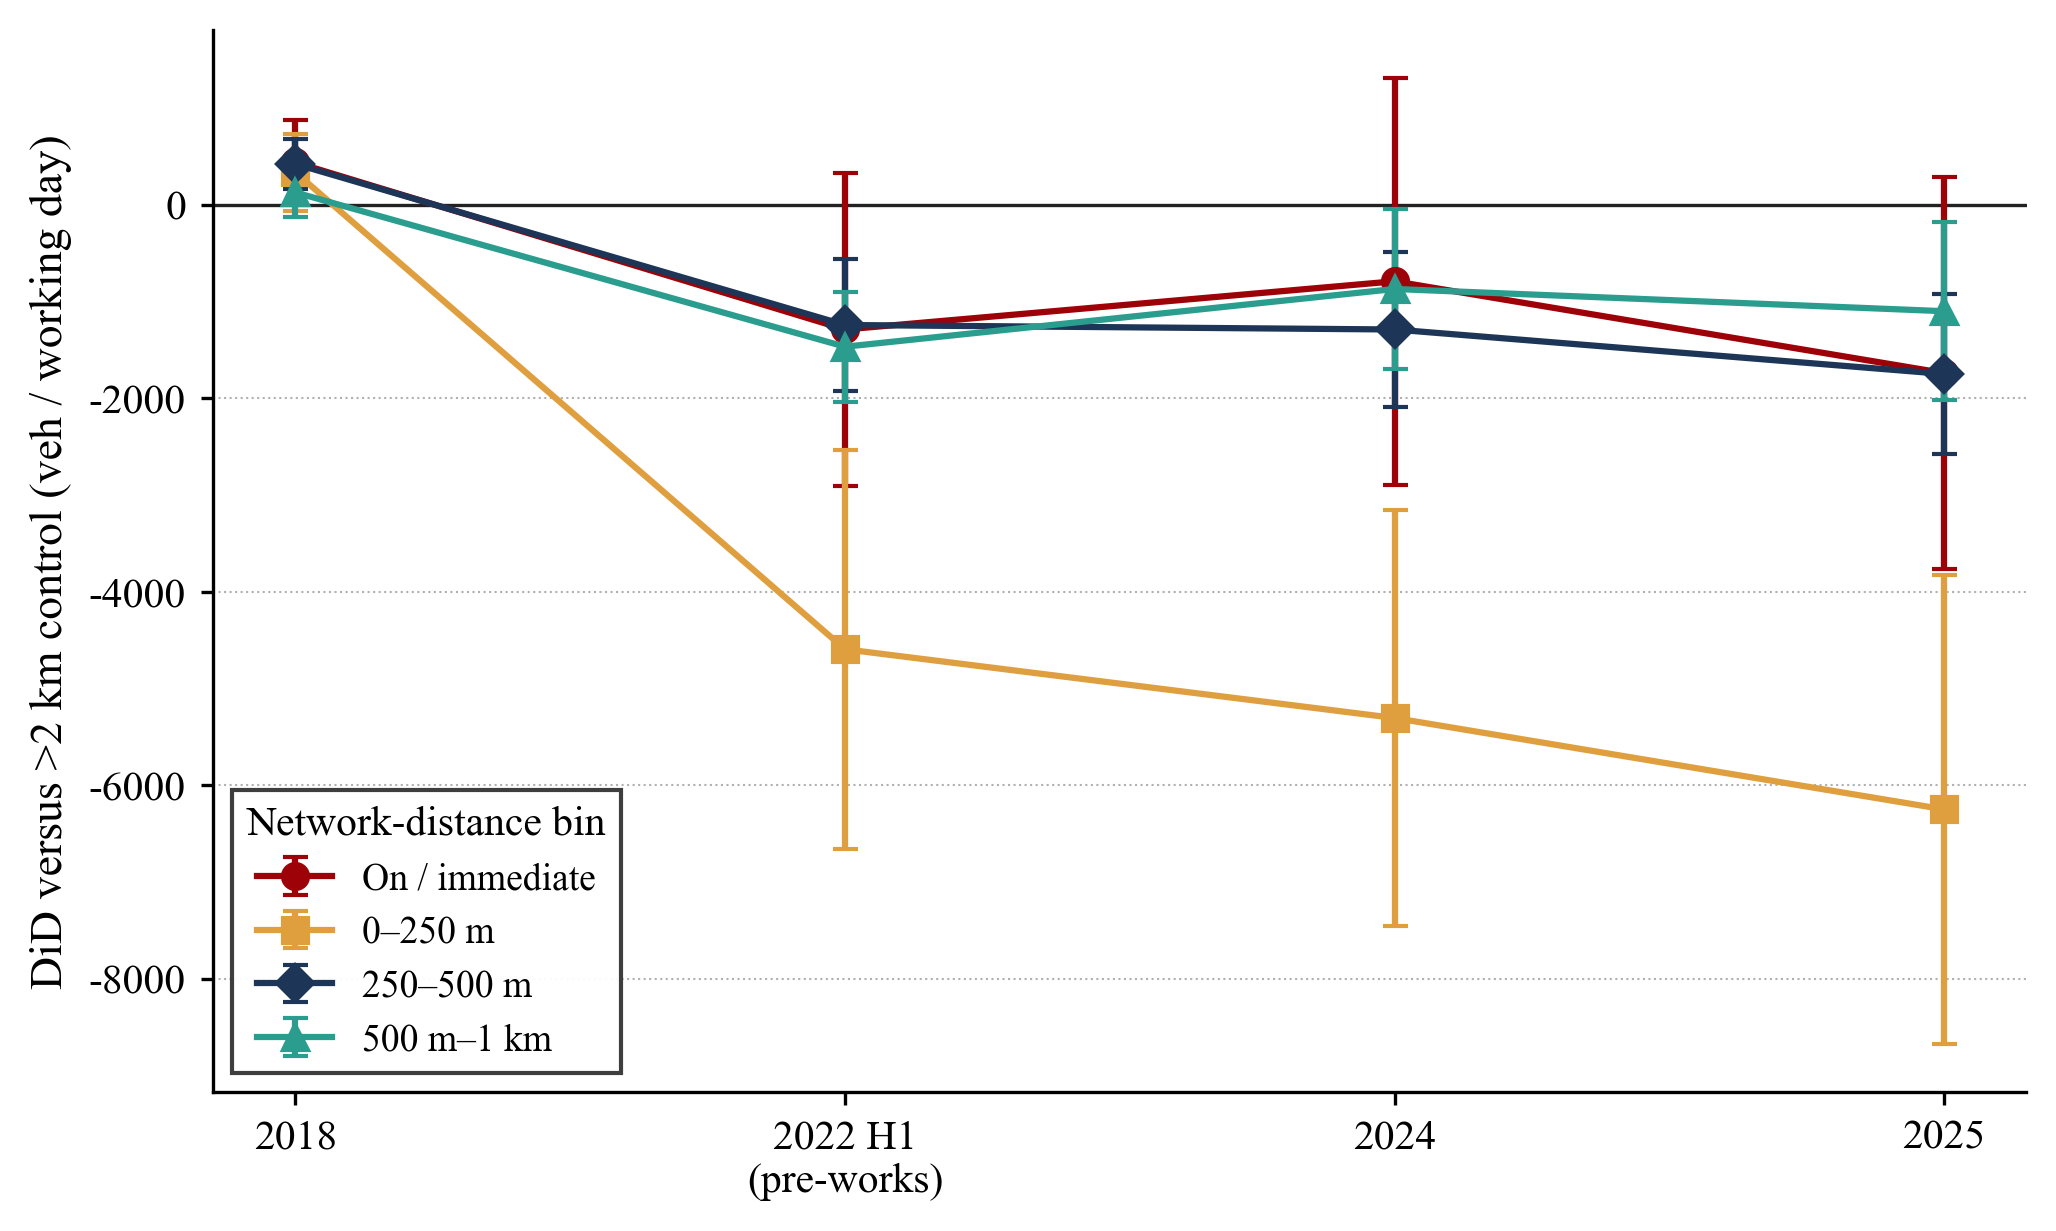
\includegraphics[width=\columnwidth]{Fig2_event_study.png}
\caption{Event-study DiD versus 2019, working-day MADT, by network-distance
bin versus stations more than 2\,km from the axes. Error bars: HC1.}
\label{fig:event}
\end{figure}

Fig.~\ref{fig:stack} plots Table~\ref{tab:cum} against the drop-2020 and
incremental specifications. After dropping 2020 counted streets that are not
the 2022 axes, no inner bin is a precise extra reduction
(Table~\ref{tab:robust}). On/immediate changes sign ($n=5$). The remaining
1--2\,km drop ($-1{,}795$, SE 722) is Diagonal / Meridiana / other corridor
change, not a 2\,km green-axis footprint. Dropping Gran Via alone leaves the
0--250\,m coefficient still large ($-6{,}128$, SE 2{,}532): Arag\'o and
Val\`encia are enough.

\begin{figure}
\centering
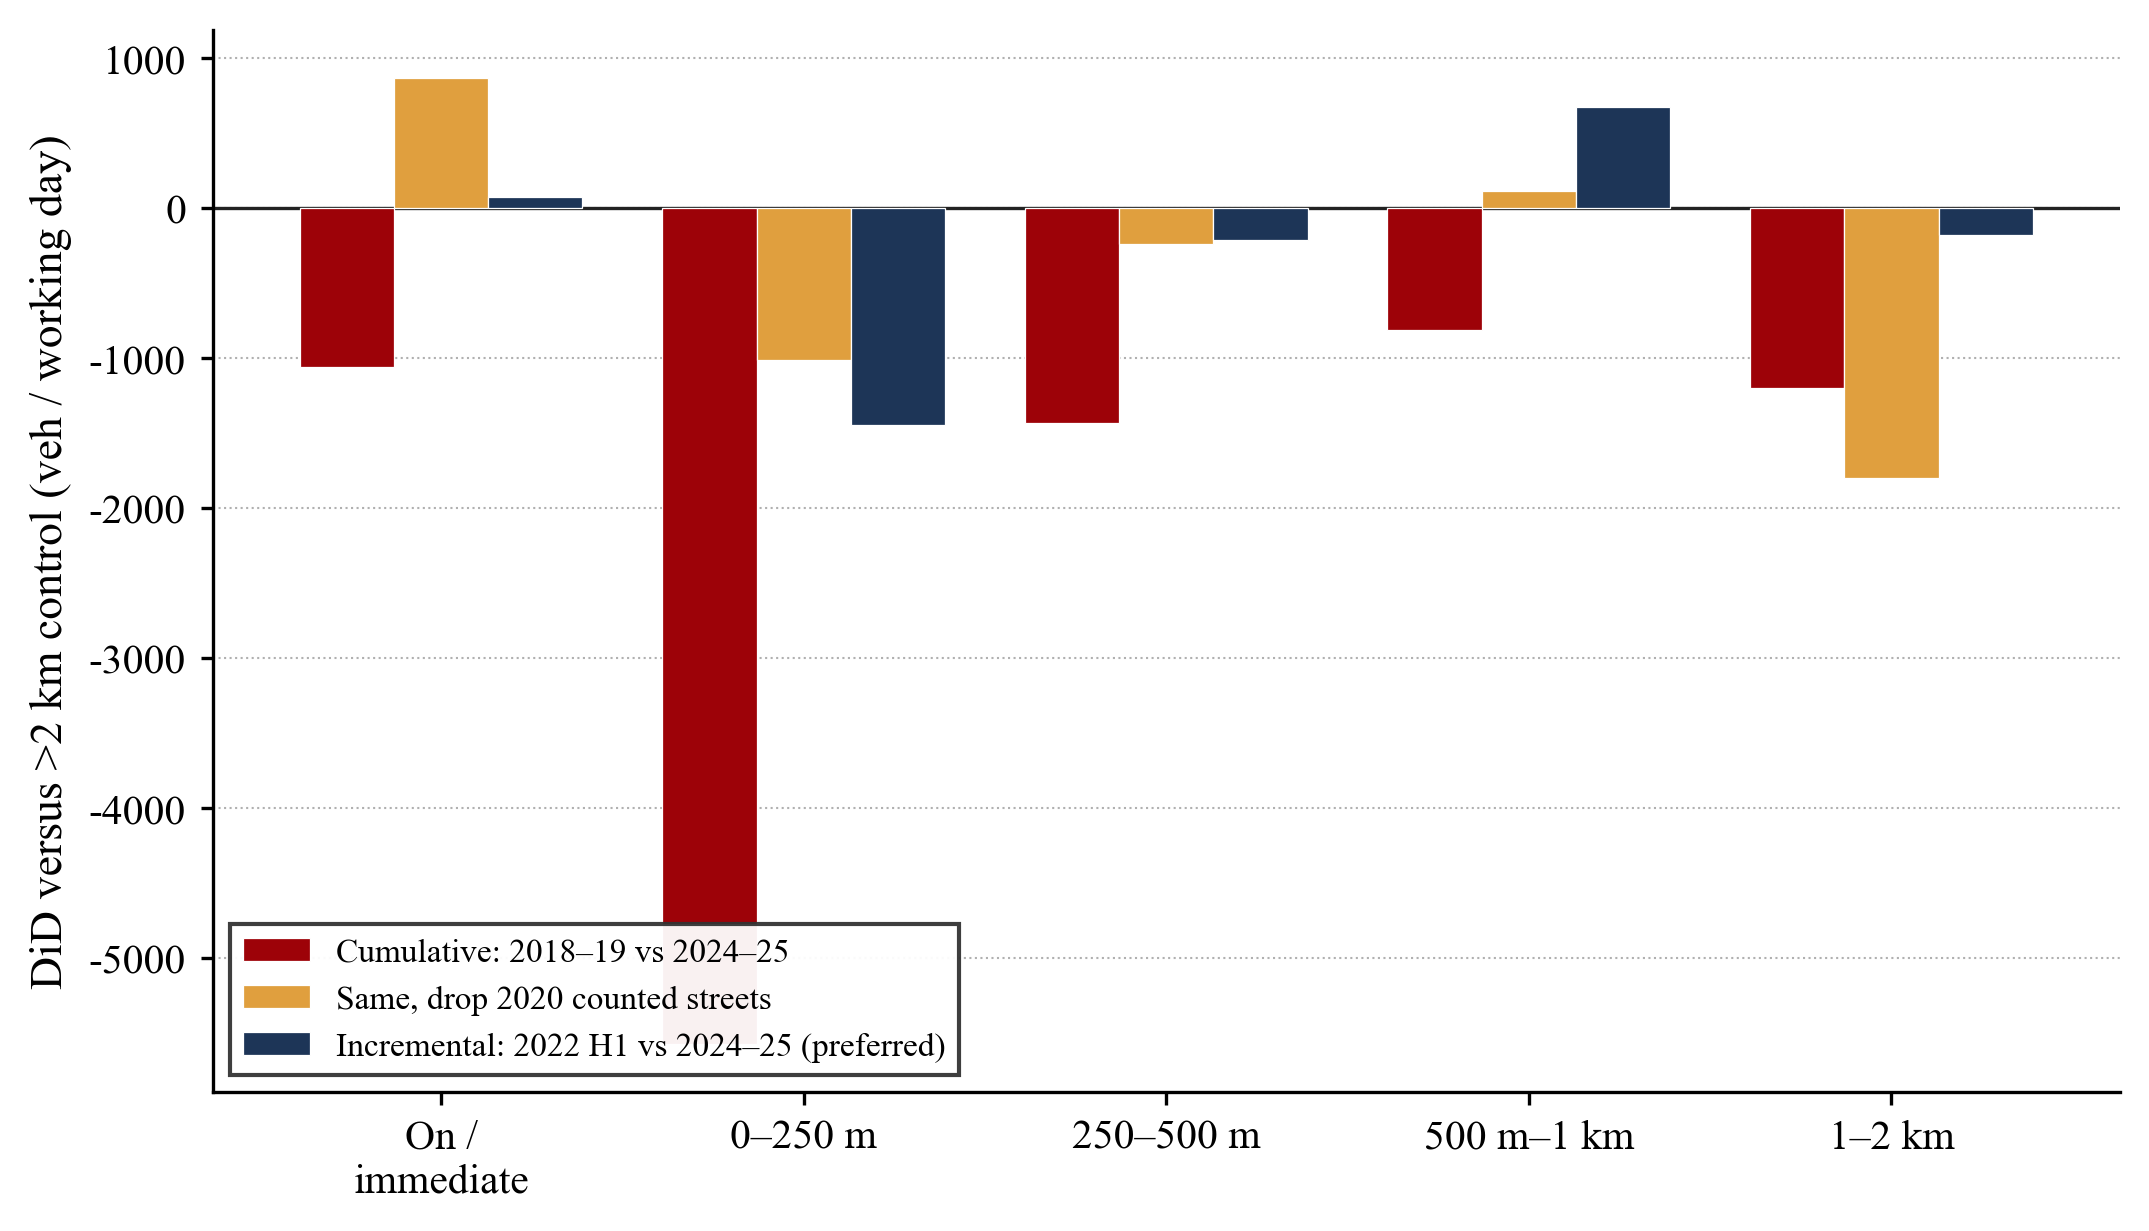
\includegraphics[width=\columnwidth]{Fig3_window_comparison.png}
\caption{DiD versus $>2$\,km under three windows: 2018--19 vs 2024--25; the
same without counted 2020 tactical streets; and 2022\,H1 vs 2024--25.}
\label{fig:stack}
\end{figure}

\begin{table}
\caption{Cumulative-window robustness, 2018--19 versus 2024--25, versus
$>2$\,km.}
\label{tab:robust}
\centering
\scriptsize
\begin{tabular}{@{}lcc@{}}
\toprule
Bin & Drop 2020 tactical & Drop Gran Via only \\
\midrule
On / immediate & $+870$ (1{,}252), $n=5$ & $-1{,}438$ (2{,}461), $n=6$ \\
0--250\,m & $-1{,}011$ (930), $n=14$ & $-6{,}128$ (2{,}532), $n=20$ \\
250--500\,m & $-239$ (715), $n=25$ & $-1{,}310$ (859), $n=33$ \\
500\,m--1\,km & $+114$ (765), $n=38$ & $-704$ (873), $n=42$ \\
1--2\,km & $-1{,}795$ (722), $n=60$ & $-1{,}698$ (700), $n=63$ \\
\bottomrule
\end{tabular}
\end{table}

\subsection{Incremental $\DQ$: the permanent-treatment window}

Table~\ref{tab:inc} and Fig.~\ref{fig:inc} are the volume result that belongs
to phase~1. Pre is January--July 2022 (tactical geometry in place, permanent
works not started). Post is 2024--25. The control marker in
Fig.~\ref{fig:inc} is at zero by construction.

\begin{table*}
\caption{Incremental DiD, 2022\,H1 versus 2024--25, versus $>2$\,km.}
\label{tab:inc}
\centering
\small
\begin{tabular}{@{}lrrrrrr@{}}
\toprule
Bin & $n$ & Pre MADT & Post MADT & Mean $\DQ$ & DiD (veh/day) & SE \\
\midrule
On / immediate & 8 & 20{,}966 & 20{,}498 & $-468$ & $\mathbf{+79}$ & 760 \\
0--250\,m & 20 & 24{,}080 & 22{,}091 & $-1{,}989$ & $\mathbf{-1{,}442}$ & 729 \\
250--500\,m & 33 & 19{,}362 & 18{,}604 & $-758$ & $\mathbf{-212}$ & 544 \\
500\,m--1\,km & 40 & 15{,}398 & 15{,}527 & $+128$ & $\mathbf{+675}$ & 579 \\
1--2\,km & 66 & 14{,}459 & 13{,}733 & $-726$ & $-180$ & 524 \\
$>2$\,km (control) & 182 & 11{,}510 & 10{,}964 & $-546$ & 0 & 151 \\
\bottomrule
\end{tabular}
\end{table*}

\begin{figure}
\centering
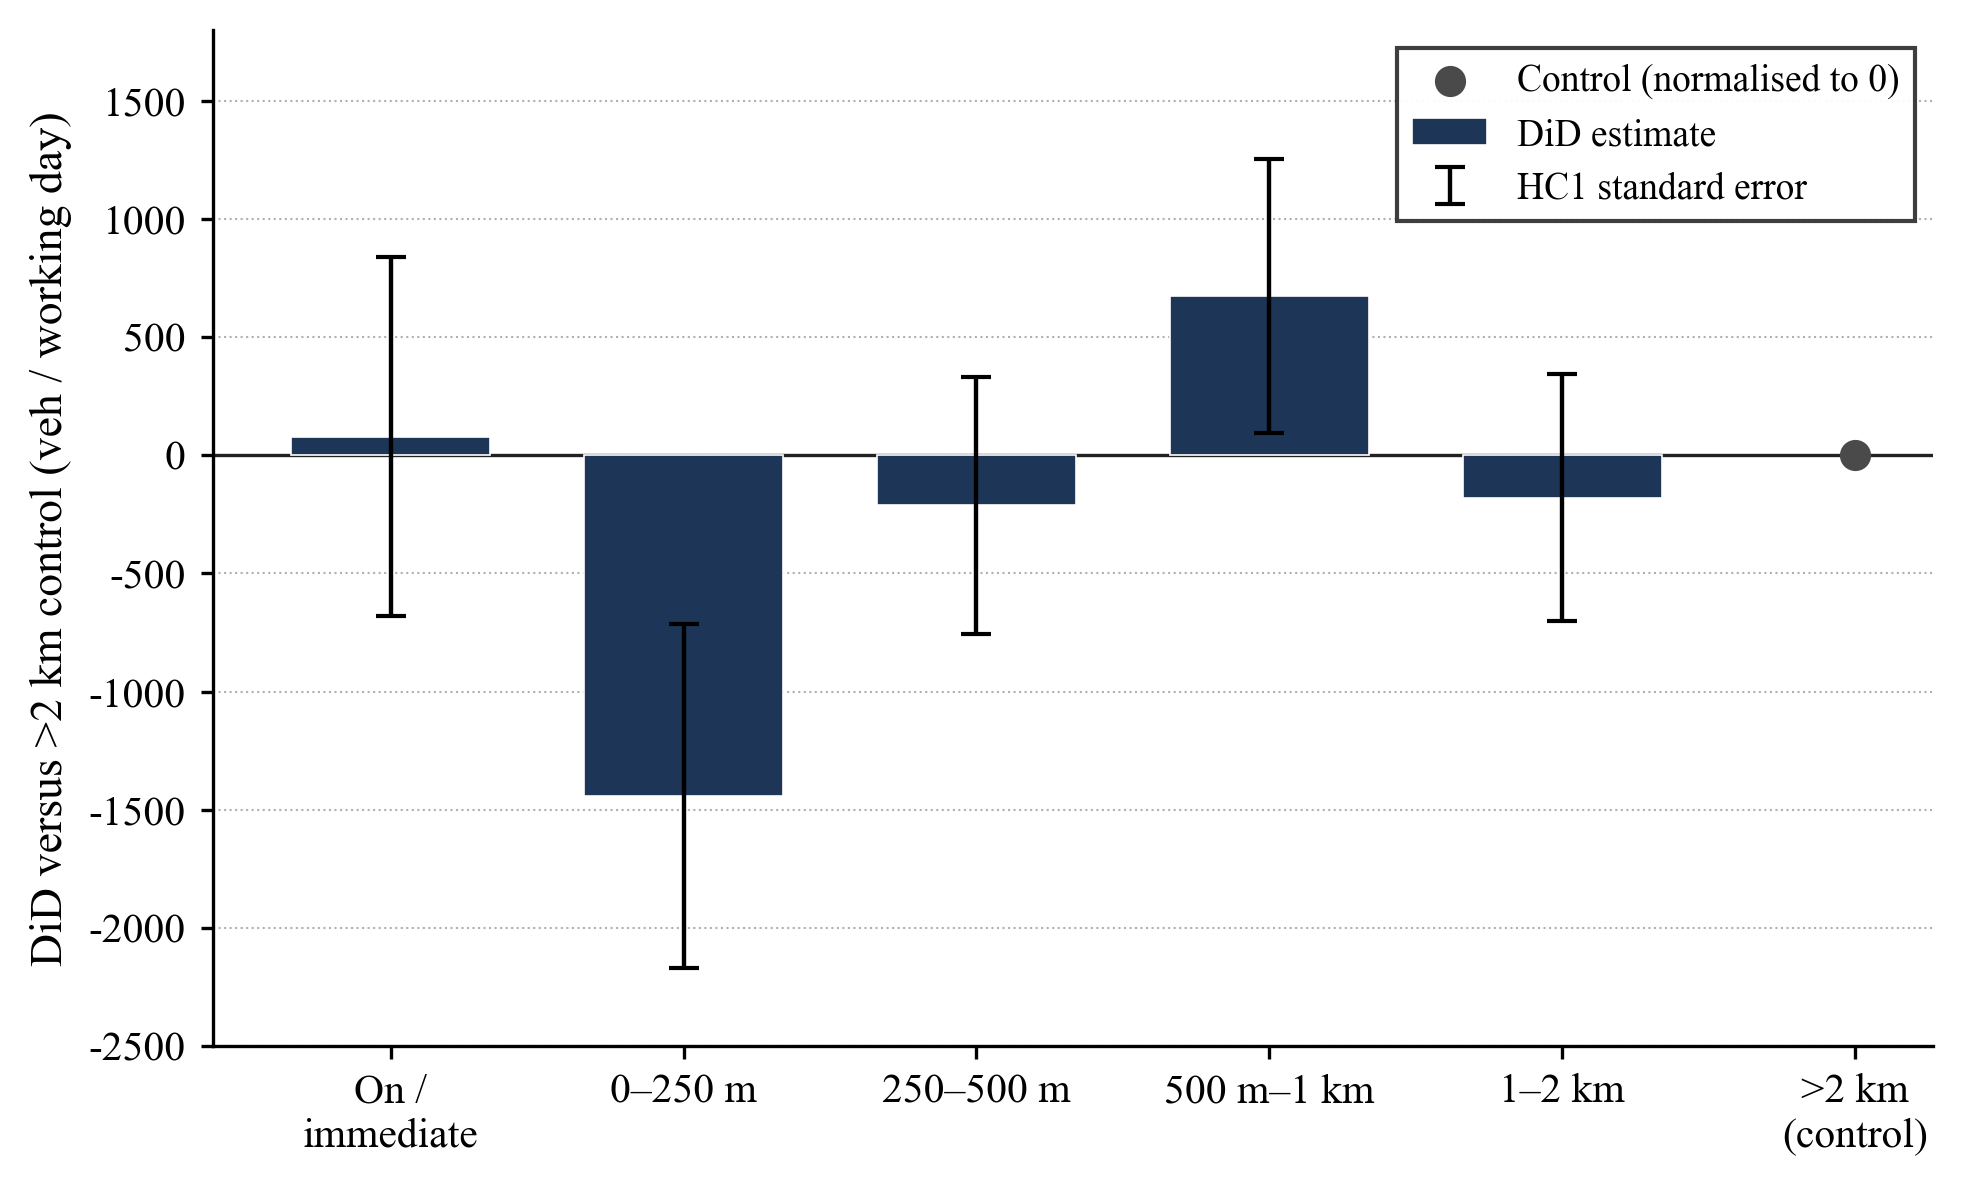
\includegraphics[width=\columnwidth]{Fig4_incremental_did.png}
\caption{Incremental DiD, 2022\,H1 versus 2024--25, versus the $>2$\,km
control. Error bars: HC1.}
\label{fig:inc}
\end{figure}

On and next to the axes, public MADT does not show a further drop once the
2020 regime is the baseline. The on/immediate DiD is $+79$ (SE 760): a
crossing-street panel, not the rebuilt pavement. Stations 4066 and 4067 remain
dark, so the simulated LTR of 39{,}597\,veh-km/day on links $\le 40$\,m is not
a counted suppression total on the new pedestrian-priority zones. Missing
on-axis MADT does not prevent the displacement test: that test is whether
surviving nearby counters rose. The 0--250\,m coefficient is about two
standard errors and is still pulled by Arag\'o and Avinguda Roma; it is not
LTR on the green-axis carriageway. The $+675$ at 500\,m--1\,km is one standard
error --- not evidence of displacement. The 250--500\,m bin, which is where a
demand-fixed model will later allocate detoured traffic, is $-212$ (SE 544)
relative to a city that itself fell by 546. Bartlett spatial HAC at 500\,m
and 1\,km and clustering on counted-street name leave that 250--500\,m
coefficient at $-212$ (SE 554, 560 and 602). Alternative network-distance
bins of 0--200, 200--400 and 400--700\,m are all negative ($-1{,}078$,
$-703$, $-272$; HC1). Restricting post to January--July 2024--25, so both
windows use the same months, leaves the 250--500\,m DiD at $-15$ (SE 479,
$n=29$). The nearby non-surge is not an artefact of HC1, of the 250/500\,m
cut-points, or of comparing a half-year pre with a full-year post.

Table~\ref{tab:inc} is the spatial pattern of observed volume change that the
assignment has to match. It is neither a measure of evaporation nor a
conversion of bin means into NVTR.

\subsection{Simulated demand-fixed LTR / NR / NVTR}

If every trip stays on the network and only routes change, the assignment
inside the 3.5\,km graph produces Table~\ref{tab:decomp} and
Fig.~\ref{fig:decomp}.

\begin{table}
\caption{Simulated demand-fixed decomposition, 3.5\,km graph (veh-km /
working day). Negative NVTR: detours add more kilometres than the local cut
removes. Not a measured saving.}
\label{tab:decomp}
\centering
\small
\begin{tabular}{@{}lrl@{}}
\toprule
Quantity & Value & Label \\
\midrule
LTR (links $\le 40$\,m) & 39{,}597 & simulated \\
NR (all other links) & $+46{,}906$ & simulated \\
NVTR $=$ LTR $-$ NR & $\mathbf{-7{,}309}$ & simulated; not measured \\
Pre network VKT & 6{,}881{,}281 & simulated \\
Post network VKT & 6{,}888{,}590 & simulated \\
\bottomrule
\end{tabular}
\end{table}

\begin{figure}
\centering
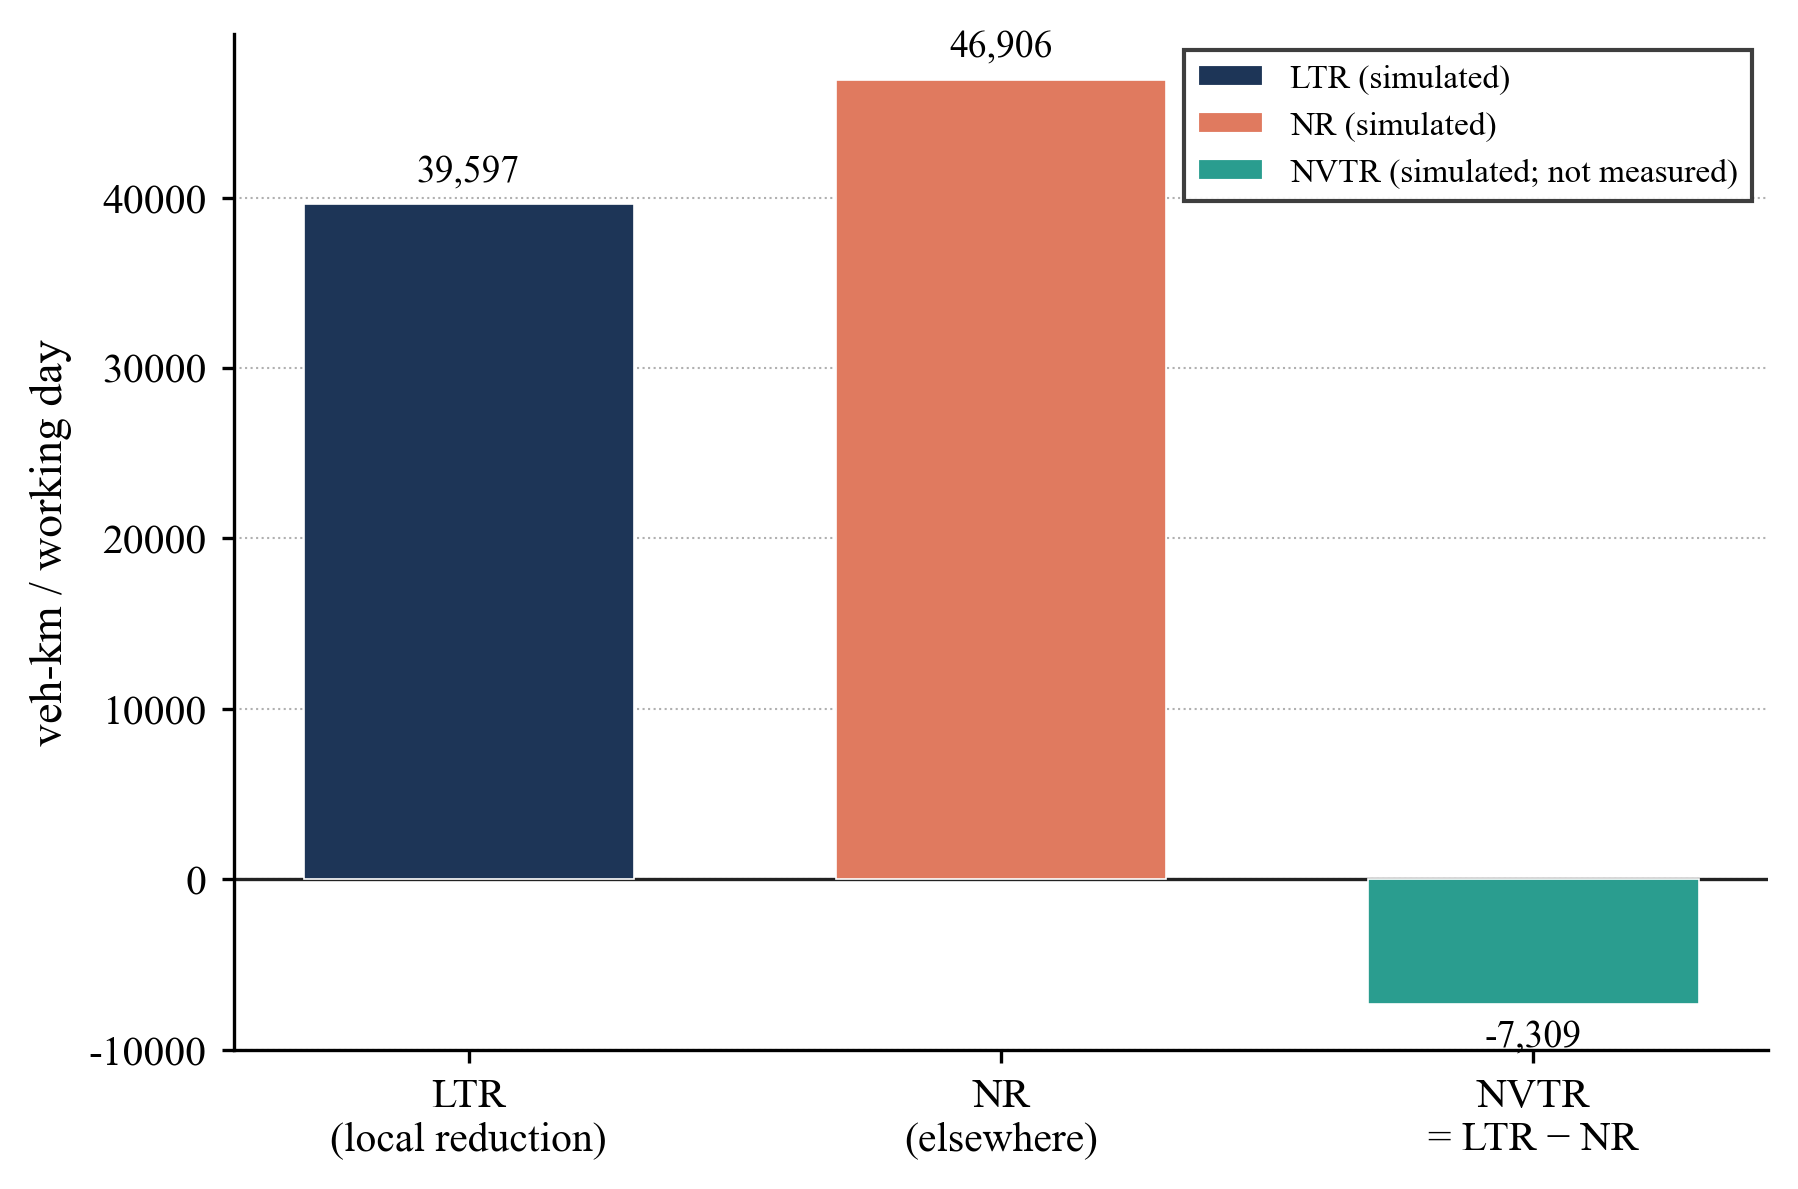
\includegraphics[width=\columnwidth]{Fig5_ltr_nr_nvtr.png}
\caption{Simulated demand-fixed LTR, NR and NVTR, 3.5\,km graph.}
\label{fig:decomp}
\end{figure}

Network VKT would \emph{rise} by about 0.1\%. Detours are longer than the cut.
Table~\ref{tab:rings} and Fig.~\ref{fig:rings} locate that extra travel: 95\%
of $|\DVKT|$ is inside 500\,m of the axes. The 250--500\,m ring is where most
of the extra vehicle-kilometres land ($+25{,}922$); 40--250\,m also gains
($+16{,}539$). The 500\,m figure is a simulated mobility-footprint radius
under demand-fixed routing. It is not an observed radius from
Table~\ref{tab:inc}.

\begin{table}
\caption{Simulated demand-fixed $\DVKT$ by network ring (veh-km / working
day).}
\label{tab:rings}
\centering
\small
\begin{tabular}{@{}lr@{}}
\toprule
Ring & $\DVKT$ \\
\midrule
0--40\,m & $-39{,}597$ \\
40--250\,m & $+16{,}539$ \\
250--500\,m & $+25{,}922$ \\
500\,m--1\,km & $+3{,}883$ \\
1--2\,km & $+562$ \\
2--3.5\,km & 0 \\
\bottomrule
\end{tabular}
\end{table}

Simulated $\DVKT$ is exactly zero on links 2--3.5\,km from the axes. On this
OSM extract, NVTR inside 2\,km therefore equals NVTR inside the 3.5\,km
boundary: enlarging $B$ cannot add simulated load that is not already on the
graph. A 4--5\,km extract is not used. Observed mean $\DQ$ beyond 2\,km is
$-546$ (Table~\ref{tab:inc}) and $-640$ at the snapped assignment stations
(Table~\ref{tab:obssim}). That citywide decline is the control, not a split of
leakage versus suppression.

\begin{figure}
\centering
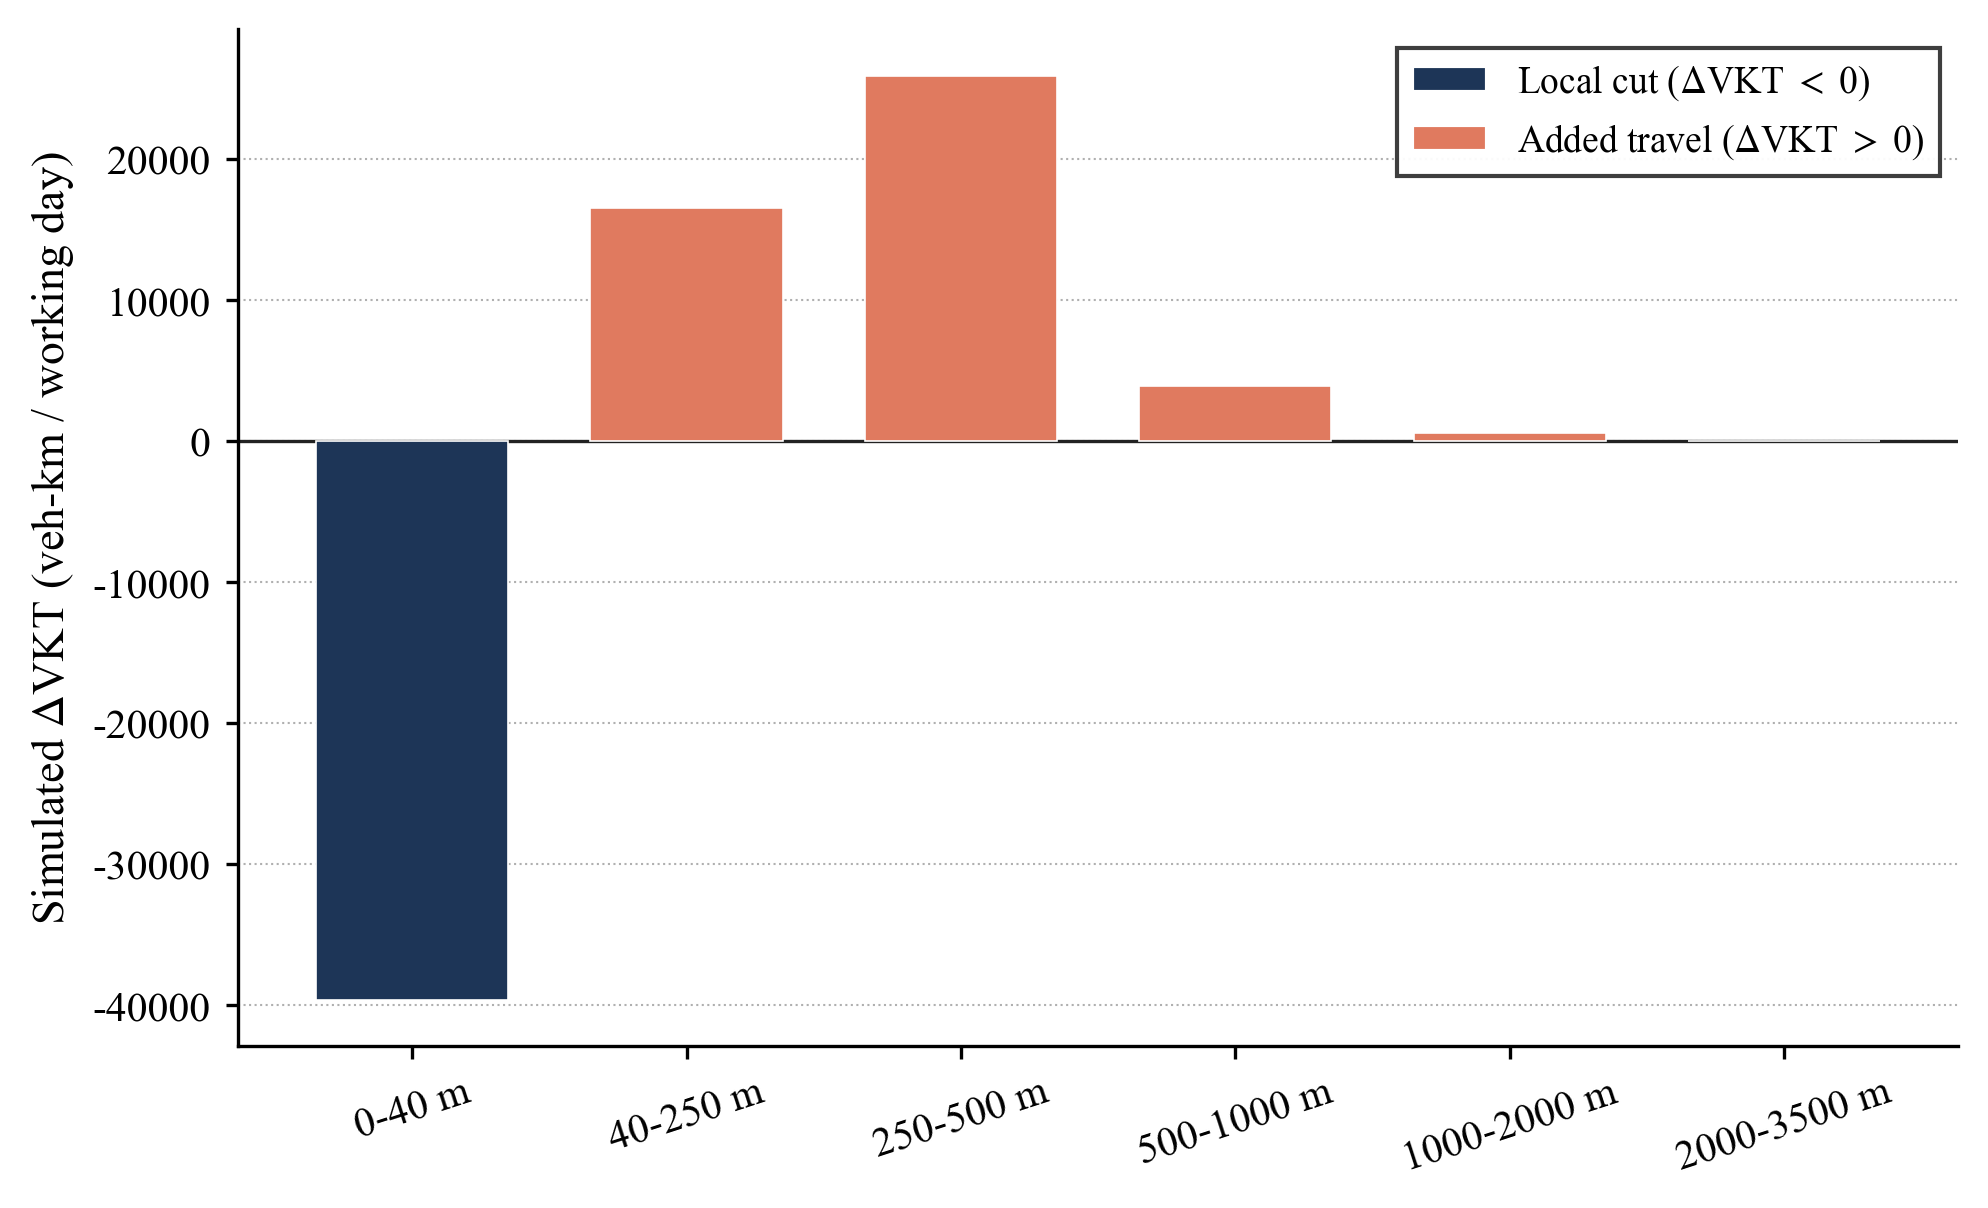
\includegraphics[width=\columnwidth]{Fig6_dvkt_by_ring.png}
\caption{Simulated demand-fixed $\DVKT$ by network ring.}
\label{fig:rings}
\end{figure}

These numbers are the demand-fixed counterfactual. They are not a measured
NVTR.

\subsection{The constraint: observed counts reject that counterfactual}

Table~\ref{tab:obssim} and Fig.~\ref{fig:obssim} compare mean incremental
$\DQ$ at snapped stations with the demand-fixed prediction.

\begin{table}
\caption{Observed incremental $\DQ$ versus simulated demand-fixed $\DQ$
(veh / working day).}
\label{tab:obssim}
\centering
\scriptsize
\begin{tabular}{@{}lrrrr@{}}
\toprule
Bin & $n$ & Obs. & Sim.\ fixed & Residual \\
\midrule
On / immediate & 8 & $-468$ & $\mathbf{-354}$ & $-114$ \\
0--250\,m & 20 & $-1{,}989$ & $-2{,}453$ & $+464$ \\
250--500\,m & 33 & $-758$ & $\mathbf{+1{,}700}$ & $\mathbf{-2{,}458}$ \\
500\,m--1\,km & 40 & $+128$ & $+131$ & $-3$ \\
1--2\,km & 66 & $-726$ & $-118$ & $-608$ \\
$>2$\,km & 130 & $-640$ & 0 & $-640$ \\
Obs.\ mean vs $+1{,}700$ & 33 & $-758$ & $+1{,}700$ & $t=-4.67$ \\
\bottomrule
\end{tabular}
\end{table}

\begin{figure}
\centering
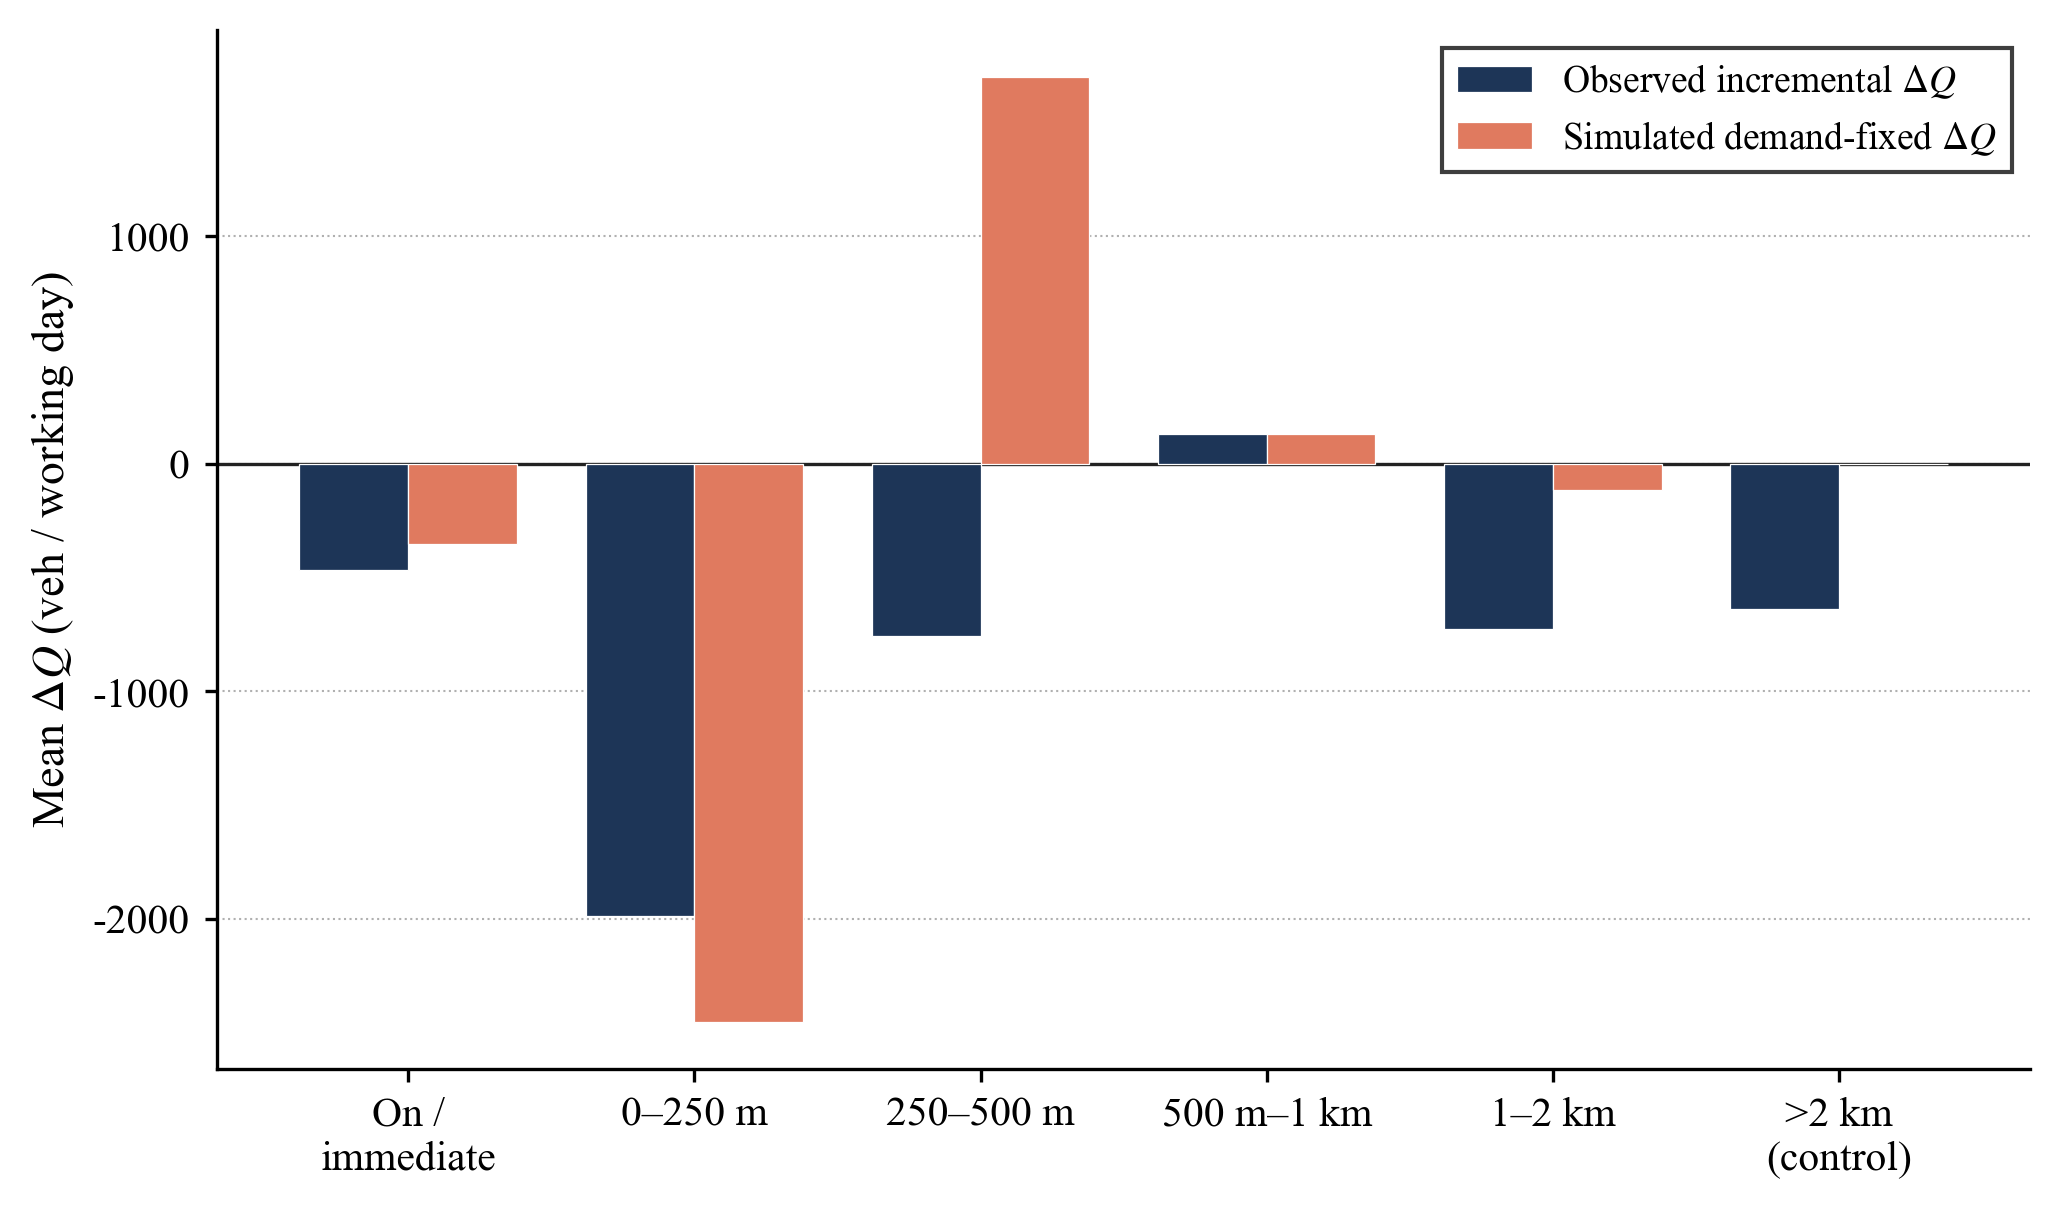
\includegraphics[width=\columnwidth]{Fig7_observed_vs_simulated.png}
\caption{Observed incremental mean $\DQ$ versus simulated demand-fixed $\DQ$
at snapped stations.}
\label{fig:obssim}
\end{figure}

Demand-fixed says the missing through-traffic should show up on counted links
250--500\,m away ($+1{,}700$). Those links track the rest of the city ($-758$
observed, versus $-640$ beyond 2\,km), not a reroute surge. Net of the
citywide residual that a fixed-OD model cannot see, the 250--500\,m gap is
still about $-1{,}800$ vehicles/day. The extra 46{,}906 veh-km in the
simulation did not appear on the instrumented network. With the as-built
centrelines on the graph, the immediate bin now has the right \emph{sign}
($-354$ simulated, $-468$ observed): flow leaves the treated links. The
rejection is the nearby surge, not the local drop. At those 33 stations the
observed mean $\DQ$ is $-758$ (SD 3{,}025, SE 527). Against the simulated
constant $+1{,}700$, $t=-4.67$ ($p<0.001$). That test is of the count
residual, not of NVTR. A DiD of $+1{,}700$ with the observed HC1 standard
error (544) would be detected at 88\% power (two-sided, $\alpha=0.05$):
the panel is not too noisy to have seen the surge.

The gravity prior, scaled only by a median factor, correlates 0.16 with
pre-period counts. Penalised GLS at $\lambda=5\times 10^{4}$ raises that to
0.59 (MAPE 0.69, RMSE 11{,}421, $n=297$) and stops at the iteration cap.
Simulated $\DQ$ magnitudes are order-of-magnitude. The \textbf{sign} at
250--500\,m is the usable result: a demand-fixed model must put extra volume
there, and the counters do not.

That sign is a property of the grid under fixed demand, not of the poorly
fitted prior. Removing through-movement on a Cerd\`a street forces remaining
OD pairs onto next-shortest paths; those paths are first parallels and
streets in the 250--500\,m ring. Gravity impedance $\beta$ changes how many
short versus long trips the prior contains. It does not reverse that
topological loading. Cost factors $\times 10$, $\times 100$ and
$\times 1{,}000$ already produce identical all-or-nothing paths
(Table~\ref{tab:spec}). Refitting origins and destinations at $\beta=1$ and
$\beta=3$ on those same paths leaves simulated $\DQ$ at 250--500\,m at
$+2{,}408$ and $+1{,}452$ (primary $\beta=2$: $+1{,}700$). A gravity-only
scale, GLS at $\lambda \in \{5\times 10^{3},5\times 10^{4},5\times 10^{5}\}$,
and 80 optimiser iterations all keep that simulated change positive
($+2{,}014$ to $+1{,}283$; Table~\ref{tab:spec}, Panel~D). Observed $\DQ$
there remains $-758$. Weak spatial fit can distort how large the simulated
surge is. It does not create the surge, and it does not explain why the
counters fail to show one.

Uniform junction delays rewrite the \emph{pre} graph. An 80\,m extra-arm
delay already removes the axes from all 2{,}307 all-or-nothing paths before
the policy penalty, so it is not a post-treatment check. Delays of 5\,m and
10\,m leave 26 and 24 OD pairs on the axes; the leftover reroute does not
reproduce the length-only $+1{,}700$ loading at the counted 250--500\,m
stations (simulated $\DQ$ $-780$ and $+2$). Cost factors
$\times 10$--$\times 1{,}000$, which isolate the forced-turn without
emptying the pre network, leave the $+1{,}700$ unchanged. Turn penalties
can move simulated leftover flow across rings. They do not produce a
counted nearby surge.

Putting the missing Consell de Cent centreline back on the graph multiplies
\emph{both} LTR and NR; NVTR stays a $\sim 0.1\%$ rise
(Table~\ref{tab:spec}). The immediate-bin simulation changes sign, from an
OSM-stub artefact ($+658$) to a local drop ($-354$). The 250--500\,m rejection
does not.

Table~\ref{tab:spec} collects the assignment specification and the geometry
and impedance checks. Assignment rows are simulated except the observed
$\DQ$ line.

\begin{table*}
\caption{Assignment specification and geometry robustness.}
\label{tab:spec}
\centering
\scriptsize
\begin{tabular}{@{}p{4.4cm}p{5.6cm}p{5.2cm}@{}}
\toprule
\multicolumn{3}{@{}l}{\emph{Panel A. Count-constrained assignment (as-built 4.85\,km)}} \\
\midrule
Item & Value & Label \\
Zones & 53 \emph{barris} & gravity prior $T_{ij} \propto P_i P_j / d_{ij}^{2}$ \\
Count-fit stations & 297 & 2022\,H1 working-day MADT \\
Correlation / MAPE / RMSE & 0.59 / 0.69 / 11{,}421 & penalised GLS on gravity prior \\
GLS ($\lambda=5\times 10^{4}$, $\le 25$ iter.) & stopped at iteration cap; 70/297 stations unhit & magnitudes order-of-magnitude \\
Origin / dest.\ log-factors & $[-4.45,2.82]$ / $[-3.50,1.94]$ & 53 zones; 2{,}307 OD pairs \\
Treated-cost $\times 10$, $\times 100$, $\times 1{,}000$ & identical AON paths & once the axis is dearer than any grid detour \\
Elastic OD refit & discarded (corr.\ 0.29) & not identified \\
Simulated footprint (80\% of $|\DVKT|$) & 500\,m (94.8\% at 500\,m) & simulation property, not DiD \\
\midrule
\multicolumn{3}{@{}l}{\emph{Panel B. Leftover OSM stubs versus as-built principal centrelines}} \\
\midrule
 & OSM stubs (2.58\,km) & As-built principal (4.85\,km, injected) \\
Directed treated km & 2.58 & 12.11 \\
LTR (veh-km/day) & 8{,}666 & 39{,}597 \\
NR (veh-km/day) & $+15{,}725$ & $+46{,}906$ \\
NVTR (veh-km/day) & $-7{,}059$ & $-7{,}309$ \\
Simulated $\DQ$, on / immediate & $+658$ & $-354$ \\
Simulated $\DQ$, 250--500\,m & $+3{,}624$ & $+1{,}700$ \\
Observed $\DQ$, 250--500\,m & $-758$ & $-758$ \\
Pre-fit correlation & 0.56 & 0.59 \\
\midrule
\multicolumn{3}{@{}l}{\emph{Panel C. Gravity impedance $\beta$ on the same pre/post paths}} \\
\midrule
Gravity $\beta$ & Pre-fit corr.\ / MAPE & Sim.\ $\DQ$ at 250--500\,m \\
1 & 0.61 / 0.68 & $+2{,}408$ (positive) \\
2 (primary) & 0.59 / 0.69 & $+1{,}700$ (positive) \\
3 & 0.54 / 0.72 & $+1{,}452$ (positive) \\
Observed $\DQ$, 250--500\,m & --- & $-758$ \\
\midrule
\multicolumn{3}{@{}l}{\emph{Panel D. Count-fit and junction delay (sign at 250--500\,m; not a new NVTR)}} \\
\midrule
Count-fit & Pre-fit corr.\ / MAPE & Sim.\ $\DQ$ at 250--500\,m \\
Gravity + median scale only & 0.16 / 1.56 & $+2{,}014$ (positive) \\
GLS $\lambda=5\times 10^{3}$, 25 iter. & 0.59 / 0.69 & $+1{,}739$ (positive) \\
GLS $\lambda=5\times 10^{4}$, 25 iter.\ (primary) & 0.59 / 0.69 & $+1{,}700$ (positive) \\
GLS $\lambda=5\times 10^{5}$, 25 iter. & 0.58 / 0.69 & $+1{,}810$ (positive) \\
GLS $\lambda=5\times 10^{4}$, 80 iter. & 0.62 / 0.66 & $+1{,}283$ (positive) \\
Junction delay 5\,m/arm & 0.53 / 0.74 & $-780$ (26 OD pairs on-axis in pre) \\
Junction delay 10\,m/arm & 0.52 / 0.80 & $+2$ (24 OD pairs on-axis in pre) \\
Junction delay 80\,m/arm & 0.46 / 0.99 & $0$ (axes unused in pre) \\
Observed $\DQ$, 250--500\,m & --- & $-758$ \\
\bottomrule
\end{tabular}
\end{table*}

Both NVTR columns in Table~\ref{tab:spec} are simulated. Local
through-movement on the axes is removed by design. Under length-only
all-or-nothing routing, nearby counted links would rise; they do not. The
demand-fixed NVTR of $-7{,}309$ is therefore not the observed network
outcome inside $B$. The residual is a mixture of trip suppression, mode
shift, destination change, retiming, leakage outside $B$, and assignment
error.

%==============================================================================
\section{Discussion}
\label{sec:disc}
%==============================================================================

\subsection{Interpretation}

Phase~1 is a forced-turn geometry plus four squares. Public on-axis series
4066 and 4067 cease after reconstruction, so LTR on the rebuilt
pedestrian-priority carriageway comes from the assignment (39{,}597\,veh-km/day
on links $\le 40$\,m), not from a post-rebuild loop. The displacement test
uses stations that continued to report.

A length-only demand-fixed assignment on that geometry predicts a large positive $\DQ$ at
250--500\,m. Observed $\DQ$ there follows the city, not the simulation. The
incremental DiD at 500\,m--1\,km ($+675$, SE 579) is within one standard
error of zero. Crossing-street on/immediate $\DQ$ is indistinguishable from
the control ($+79$, SE 760). Localized adjacent displacement on the
instrumented 3.5\,km network is therefore not the observed pattern.

Even under the rejected demand-fixed run, local VKT falls by 39{,}597 veh-km
while network VKT would rise. Table~\ref{tab:inc} and Table~\ref{tab:decomp}
are different objects.

The demand-fixed model allows only rerouting. Disappearing traffic is a
bundle of route, time, destination, mode and trip-frequency responses
\citep{Cairns2002}; reduced demand is the capacity-removal counterpart of
induced travel \citep{SACTRA1994,Goodwin1996}. On a dense grid, removing a
link need not produce severe parallel congestion
\citep{Braess1968,Downs1962,Thomson1977}. \citet{Tennoy2021} document the
empirical analogue: remaining-link volumes fell while congestion rose, and
travellers changed route, time and mode. The Barcelona counts are consistent
with that catalogue. They do not split the residual into suppression, mode
shift, retiming, destination change or leakage beyond $B$. Leakage here
includes macro-rerouting onto the Ronda Litoral or Ronda de Dalt: those
ring roads sit outside the 3.5\,km graph, so a trip that leaves $B$ for a
Ronda is observationally equivalent, from inside this assignment, to a trip
that left the car. Widening $B$ until it contains the Rondes would be a
different system boundary and a different paper. Simulated $\DVKT$ is already
zero in the 2--3.5\,km ring on the present extract, so leftover flow is not
sitting in that outer ring waiting to be counted.

The 2018--19 versus 2024--25 nearby drop is the 2020 arterial programme
(Arag\'o, Val\`encia, Gran Via). The incremental window isolates phase~1 from
that earlier cut. Low-emission-zone rules and metropolitan transit fares in
2022--25 apply across the municipality. The $>2$\,km control differences those
common shocks to the extent they load the Eixample and the rest of the city
equally. A more central bite than the control would pull nearby DiD down; it
would not, by itself, produce the demand-fixed $+1{,}700$ at 250--500\,m.

\subsection{Scope of the estimates}

Citywide elastic NVTR is not identified. The gravity prior is not a
household-survey matrix; the penalised GLS adjustment hits the iteration cap
and leaves 70 of 297 stations unhit; a second OD refit to 2024--25 counts was
an artefact; and $B$ is a 3.5\,km graph, not the metropolitan system.
Simulated $-7{,}309$ is the demand-fixed counterfactual that the counts
reject: network VKT inside $B$ would \emph{rise} because detours are longer
than the cut. Simulated $\DVKT$ is zero in the 2--3.5\,km ring, so leftover flow
that left $B$ is not recovered by widening the present extract. Observed
decline beyond 2\,km ($-546$ mean $\DQ$) is consistent with a citywide drop
and does not separate leakage from suppression, retiming or mode shift.
Whether that leftover is true evaporation or VKT pushed onto the Rondes is
exactly the unidentified object.

On-axis LTR is likewise simulated. Stations 4066 and 4067 remain empty in
2023--25. Station 4056 reappears in 2025 from May, 1.07\,km network east of
phase~1, and is not treated-pavement LTR.

\subsection{Monitoring}

Before it cuts a street, a city can: (i)~instrument the network by
\textbf{network distance}, not a 500\,m circle; (ii)~keep a \textbf{pre-works
baseline after any earlier tactical regime}, so that paint and concrete are
not pooled; (iii)~report LTR, NR and NVTR from an assignment with a
\textbf{stated demand scenario}, and show the count residual; (iv)~treat a
demand-fixed NVTR that the counts contradict as a rejected counterfactual, not
as a headline saving. Health, retail and accessibility remain outside the
present objects.

\subsection{Limitations}

No observed OD: public EMEF is corona-level. Dark on-axis stations 4066 and
4067 (and 6027, 6028) after 2022, so treated-pavement LTR is simulated rather
than counted; no further on-axis loops are in the open release. Treated
geometry is the as-built 4.85\,km; directed treated length (12.11\,km) still
double-counts some parallel OSM stubs. The gravity prior, after penalised
GLS, fits counts at correlation 0.59, with 24\% of stations unhit; simulated
$\DQ$ magnitudes are order-of-magnitude, while the 250--500\,m sign stays
positive across $\beta$, $\lambda$, iteration cap and a median-scale-only
prior. Open aforaments are monthly working-day MADT, so peak-hour retiming is
not observed. Link capacities and signal timings are not in the OSM extract,
so equilibrium assignment is not estimated. Uniform extra-arm delays of
5--80\,m are a proxy, not an observed turn penalty; 80\,m already empties
the axes in the pre network. Manual Pla de Mobilitat Urbana counts are not
in the open aforament release used here and are not substituted for 4066
and 4067. The literature review is
organised around the volume-versus-VKT distinction that structures the
research question.

%==============================================================================
\section{Conclusion}
\label{sec:conc}
%==============================================================================

Road-space reallocation is advocated, and contested, as a change in how much
people drive. The data cities actually collect are how many vehicles pass a
point. This paper keeps those objects apart for Barcelona's first permanent
green axes.

On public working-day MADT, the large nearby drop between 2018--19 and
2024--25 is the 2020 arterial programme, not Eixos Verds phase~1. Relative to
2022\,H1, crossing and nearby stations do not show a further local collapse or
a precise displacement bump. A simulated, order-of-magnitude demand-fixed
assignment on the as-built 4.85\,km of phase-1 centreline would have produced
39{,}597\,veh-km/day of local reduction, 46{,}906\,veh-km of extra travel
elsewhere, a small rise in network VKT, and a surge at 250--500\,m. The
counters reject that surge.
Local through-movement was designed out; one-for-one redistribution inside
3.5\,km is not what happened on the instrumented streets. That finding is a
lack of localized adjacent displacement. It is not a measured net reduction
in citywide vehicle travel. Leftover flow may have shifted to other modes,
other hours, other destinations, or links outside the 3.5\,km graph.

Net vehicle travel for the city is still unmeasured. Until an observed
origin--destination matrix is on the graph, NVTR remains a labelled scenario,
not a statistic. The mobility-footprint procedure --- network distance, a
clean incremental window, and a count-constrained split of LTR, NR and NVTR
--- is the result that travels. The next data input tightens the number. It
does not change the question.

%==============================================================================
\section*{CRediT authorship contribution statement}
%==============================================================================

\noindent\textbf{Seshadri Naik Moode:} Conceptualization; Methodology;
Software; Formal analysis; Validation; Visualization; Writing -- original
draft; Writing -- review \& editing.

\section*{Declaration of competing interest}

The author declares that he has no known competing financial interests or
personal relationships that could have appeared to influence the work reported
in this paper.

\section*{Funding}

This research has been partially funded by the Spanish Ministry of Economy
and Competitiveness (Ministerio de Econom\'{i}a y Competitividad, Gobierno
de Espa\~{n}a), Grant ref.\ PID2019-105331RB-I00, number J-02653 Platoon.
Publications and other results are supported by the JOAN OR\'{O} FI
AGAUR-2022 grant num.\ FI\_B 00597 of the Secretariat for Universities and
Research of the Department of Research and Universities of the Generalitat
de Catalunya and the European Social Fund Plus.

\section*{Ethics statement}

This study uses publicly released traffic-count series, neighbourhood
boundaries and census population. No human-subject data were collected.
Institutional ethics approval was not required.

\section*{Data availability}

Traffic counts are from Ajuntament de Barcelona Open Data (datasets
\emph{aforaments-descriptiu} and \emph{aforaments-detall}; monthly working-day
MADT extracts for 2017--2025). Neighbourhood (\emph{barris}) boundaries and
2022 \emph{padr\'o} population are from the same portal. The street network is
OpenStreetMap motorised highways. The ATM/EMEF origin--destination matrix was
not used. Processed station-level panels, difference-in-differences tables,
assignment outputs and the Python scripts that reproduce all numbered tables
and figures are available from the corresponding author and will be deposited
in an open repository upon acceptance.

\section*{Declaration of generative AI in scientific writing}

During the preparation of this work the author used language-model assistance
(Cursor) in order to draft and edit the manuscript. After using this tool, the
author reviewed and edited the content as needed and takes full responsibility
for the content of the publication.

\bibliographystyle{cas-model2-names}
\bibliography{references}

\end{document}
